
\documentclass[11pt, a4paper]{article}
%\usepackage{proj1}
\usepackage{natbib}
\usepackage{fancyhdr}  
\usepackage{subcaption}
\usepackage{caption}
\usepackage{graphicx}
\usepackage{numprint}
\usepackage{multirow}
\linespread{1.25} 
\setlength{\parindent}{0cm}
\graphicspath{{Images/}}
\usepackage{hyperref}
\usepackage{amsmath}
\usepackage{amsfonts}
\usepackage{amssymb}
\usepackage{amsthm}
\usepackage{mathtools}
\usepackage{commath}
\usepackage{bbm}

%\usepackage[sc,osf]{mathpazo}
\usepackage{subcaption}
\usepackage[a4paper, top=1in, left=1.0in, right=1.0in, bottom=1in, includehead, includefoot]{geometry} %Usually have top as 1in

\usepackage{listings}
\usepackage{color} %red, green, blue, yellow, cyan, magenta, black, white
\definecolor{mygreen}{RGB}{28,172,0} % color values Red, Green, Blue
\definecolor{mylilas}{RGB}{170,55,241}


\hypersetup{colorlinks,linkcolor={black},citecolor={blue},urlcolor={black}}
\usepackage{color}
\urlstyle{same}


\theoremstyle{definition}
\newtheorem{definition}{Definition}[section]

\newcommand{\adja}{q_a}
\newcommand{\adjb}{q_b}
\newcommand{\adjaB}{q_{a,\partial \Omega}}
\newcommand{\adjbB}{q_{b,\partial \Omega}}
\newcommand{\adjB}{q_{\partial \Omega}}
\newcommand{\Adja}{\mathbf{p}}
\newcommand{\Adjb}{q}
\newcommand{\adj}{q}
\newcommand{\Adjc}{{q}_{\partial \Omega}}
\newcommand{\ra}{\rho_a}
\newcommand{\rb}{\rho_b}
\newcommand{\w}{\mathbf{w}}
\newcommand{\x}{\mathbf{x}}
\newcommand{\f}{\mathbf{f}}
\newcommand{\ve}{\mathbf{v}}
\newcommand{\n}{\mathbf{n}}
\newcommand{\h}{\mathbf{h}}
\newcommand{\K}{\mathbf{K}}
\newcommand{\hr}{\widehat \rho}
\newcommand{\jf}{\mathbf j}

\DeclareMathOperator{\sgn}{sgn}
\DeclareMathOperator{\Grad}{Grad}
\DeclareMathOperator{\Div}{Div}
\DeclareMathOperator{\Lap}{Lap}
%	\begin{figure}[h]
%		\centering
%		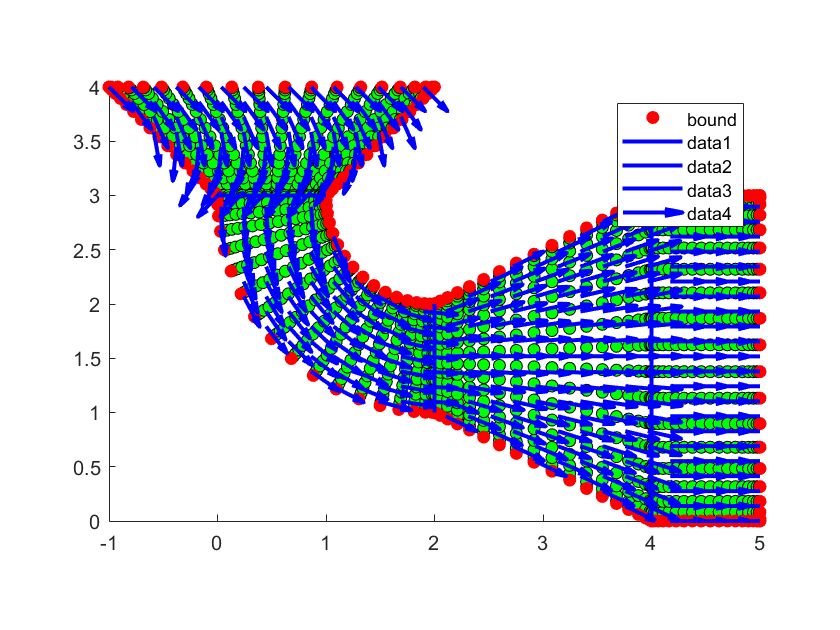
\includegraphics[scale=0.35]{F1.png}
%		\caption{Forward $\rho$ for $a = 0.01$} 
%		\label{F1}
%	\end{figure}

\begin{document}
	\section*{Paper Examples 2D}
	All the below examples are run with Newton-Krylov. They all converged within $10$ outer iterations. The baseline for the cost functional is the problem computed with $\beta = 10^3$.
	I changed the colormap to fewer colors, so that the differences between the different $\kappa$ are visible in the initial times, while also scaling the colormap for the overall maximum of $\rho$ over all times and $\kappa$.
	The controls are also scaled for all times and $\kappa$ (for flow control we use the largest value over all times and $\kappa$ as the scaling for the arrow).
	\section{Neumann Source Control}
	We choose 
	\begin{align*}
		\rho_0 &= \frac{1}{4}\\
		V_{ext} &= \frac{3}{2}\cos\left(\frac{\pi x_1}{5} - \frac{\pi}{5}\right)\sin\left(\frac{\pi x_2}{5}\right)\\
		\hr &= \frac{1}{4}(1 - t) + t\left(\frac{1}{4}\sin\left(\frac{\pi \left(x_1 - 2\right)}{2}\right)\sin\left(\frac{\pi (x_2 - 2)}{2}\right) + \frac{1}{4}\right)
	\end{align*}
	We choose the domain $[-1,1]^2$ with a time horizon $(0,1)$ and $N = 20$, $n = 11$. 
	For $\beta = 10^{-3}$, for $\kappa = -1$ we have $\mathcal J_c = 0.0018$, for $\kappa = 0$ (compared to $\mathcal J_{uc} = 0.0274$ from $\beta = 10^3$), $\mathcal J_c = 0.0017$ and for $\kappa = 1$, $\mathcal J_c = 0.0018$. Each of these computations takes around $200$ seconds for $10$ outer iterations. The results can be seen in Figures \ref{F1a}, \ref{F1b} and \ref{F1c}.\\
	We run the same example with $\beta = 10^{-5}$. This gives for $\kappa = -1$, $\mathcal J_c = 8.0673 \times 10^{-4}$, for $\kappa = 0$, $\mathcal J_c = 8.1989 \times 10^{-4}$, and for $\kappa = 1$, $\mathcal J_c = 8.4241 \times 10^{-4}$. Notably, these calculations only take around $20$ seconds. 
	

	\begin{figure}[h]
		\centering
		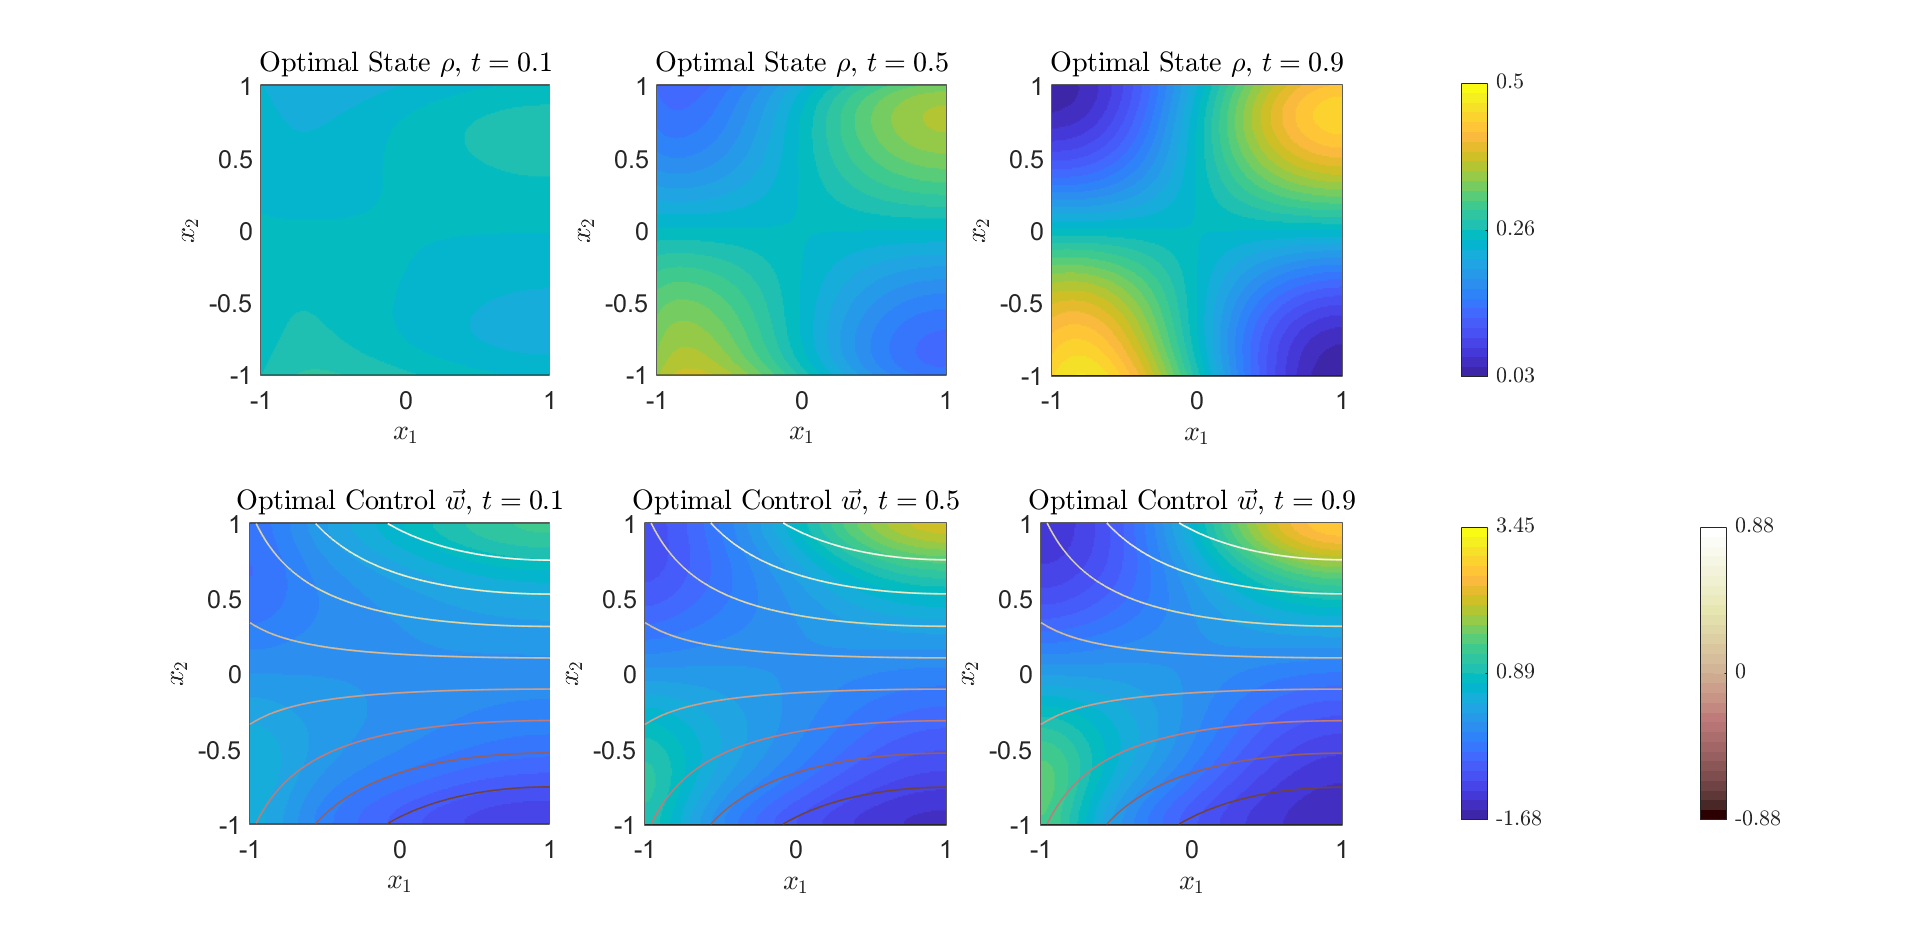
\includegraphics[scale=0.35]{SCNk0.png}
		\caption{Neumann Source Control: Optimal $\rho$ and optimal control for $\kappa = 0$ and $\beta = 10^{-3}$.} 
		\label{F1a}
	\end{figure}
	\begin{figure}[h]
		\centering
		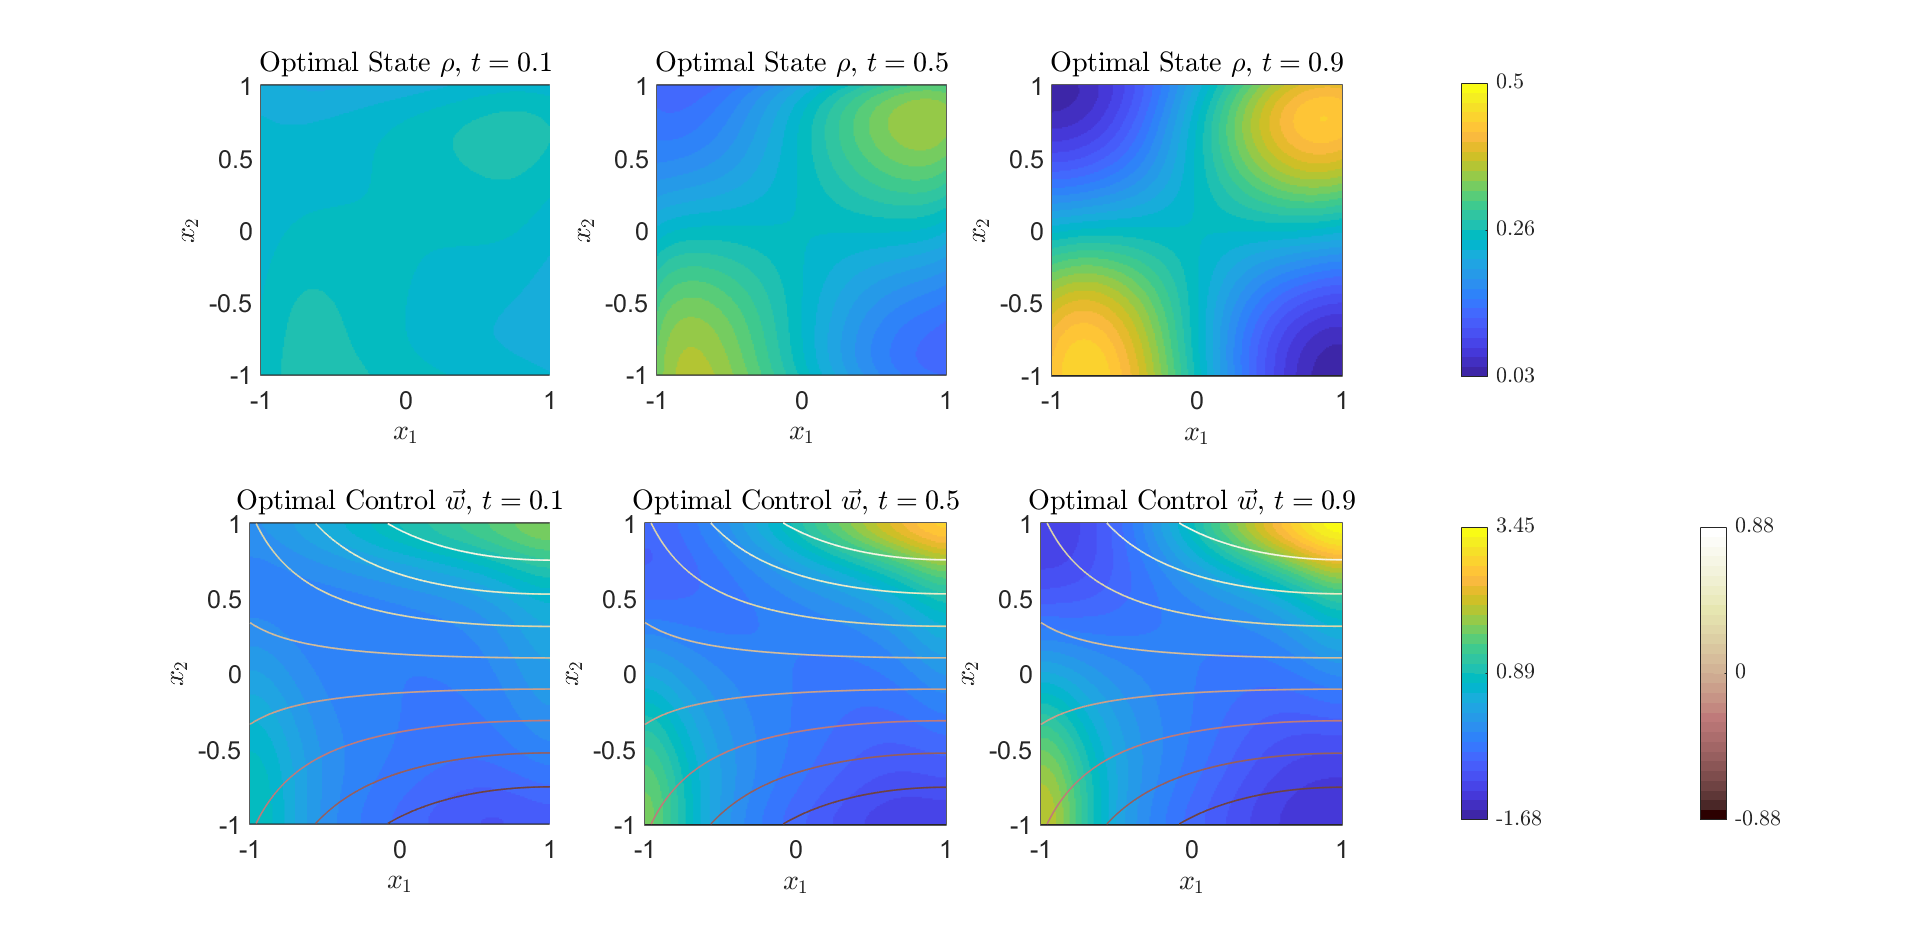
\includegraphics[scale=0.35]{SCNkn1.png}
		\caption{Neumann Source Control: Optimal $\rho$ and optimal control for $\kappa = -1$ and $\beta = 10^{-3}$.} 
		\label{F1b}
	\end{figure}
	\begin{figure}[h]
		\centering
		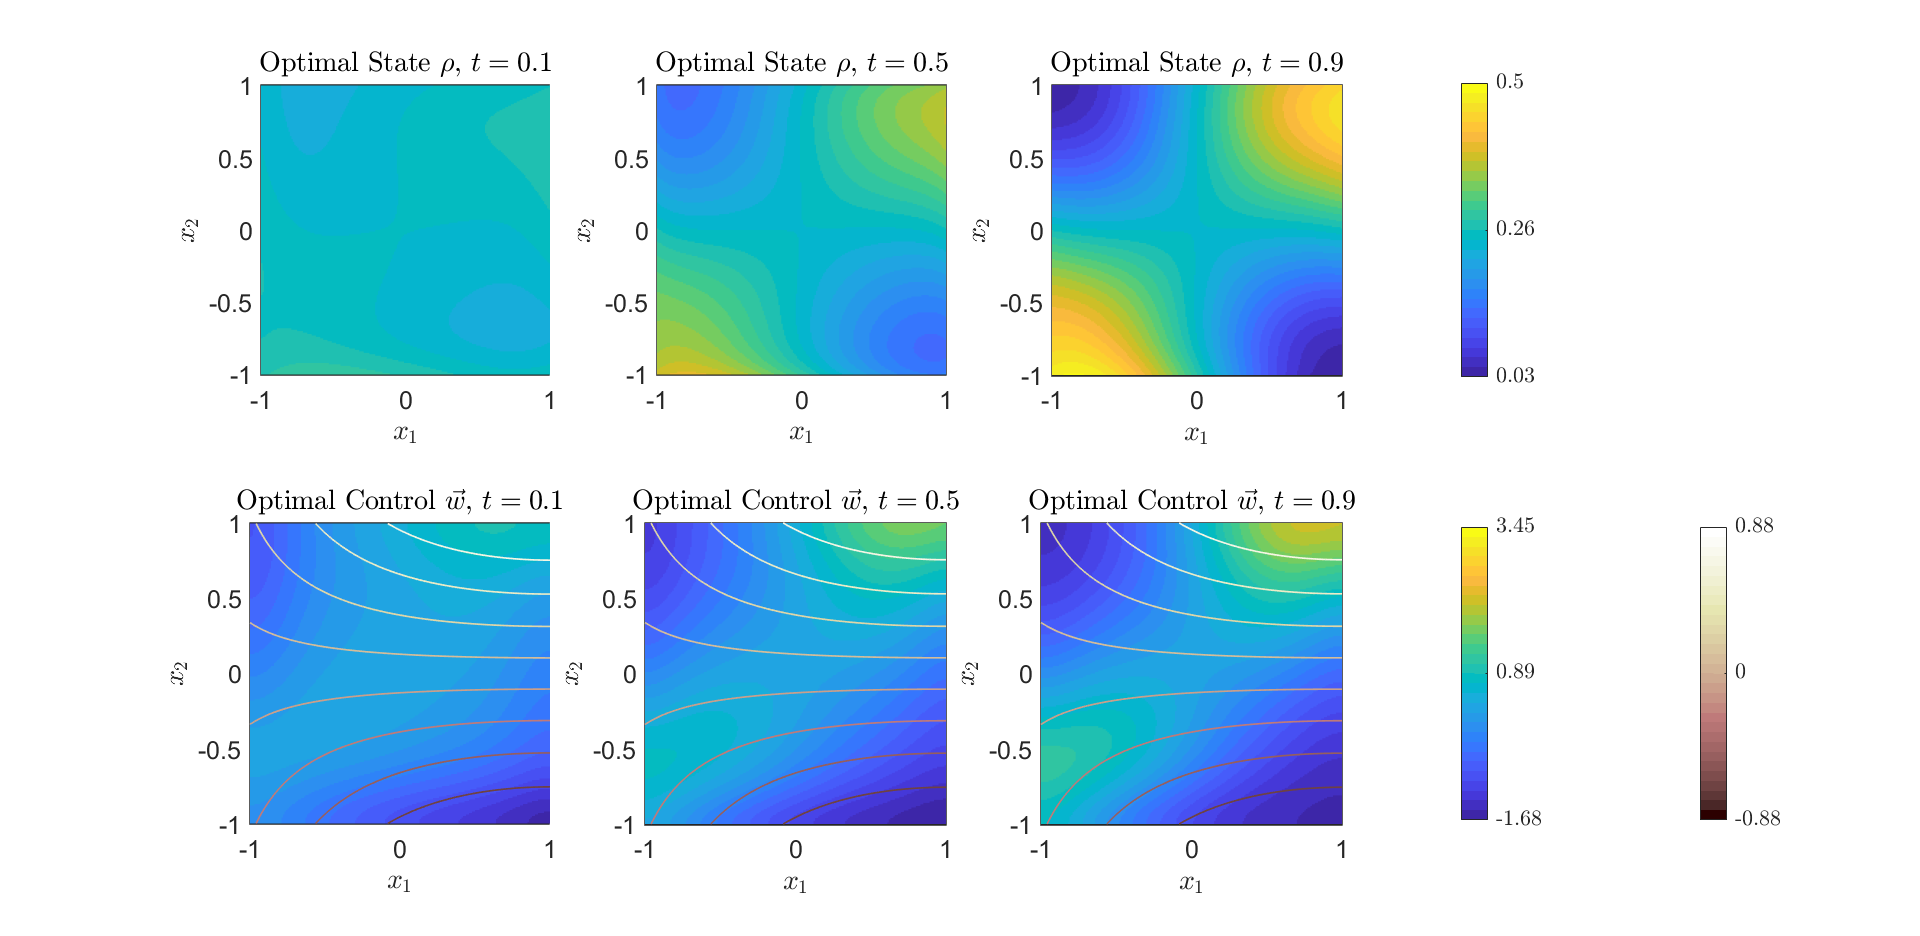
\includegraphics[scale=0.35]{SCNk1.png}
		\caption{Optimal $\rho$ and optimal control for $\kappa = 1$ and $\beta = 10^{-3}$.} 
		\label{F1c}
	\end{figure}

	\section{Dirichlet Source Control}
	We choose 
	\begin{align*}
		\rho_0 &= \frac{1}{4}\cos\left(\frac{\pi x_1}{2}\right)\cos\left(\frac{\pi x_2}{2}\right) + \frac{1}{4}\\
		V_{ext} &=  2(1-t)\left(-\cos\left(\frac{\pi x_1}{2}\right)\sin\left(\frac{\pi x_2}{2}\right) + 1\right)\\
		\hr &= (1 - t)\left(\frac{1}{4}\cos\left(\frac{\pi x_1}{2}\right)\cos\left(\frac{\pi x_2}{2}\right) + \frac{1}{4}\right) - t\left(\frac{1}{4}\sin\left(\pi x_1\right)\sin\left(\frac{\pi x_2}{2} - \frac{\pi}{2}\right) + \frac{1}{4}\right)
	\end{align*}
	so that the problem has Dirichlet boundary conditions at $0.25$ ($\rho = 0.25$ on $\partial \Omega$).
	We choose the domain $[-1,1]^2$ with a time horizon $(0,1)$ and $N = 20$, $n = 11$.
	For $\beta = 10^{-3}$, for $\kappa = -1$ we have $\mathcal J_c = 0.0036$, for $\kappa = 0$ (compared to $\mathcal J_{uc} = 0.0219$ from $\beta = 10^3$), $\mathcal J_c = 0.0038$ and for $\kappa = 1$, $\mathcal J_c = 0.0043$. Each of these computations takes around $70$ seconds for $10$ outer iterations. The results can be seen in Figures \ref{F2a}, \ref{F2b} and \ref{F2c}.\\
	

	\begin{figure}[h]
		\centering
		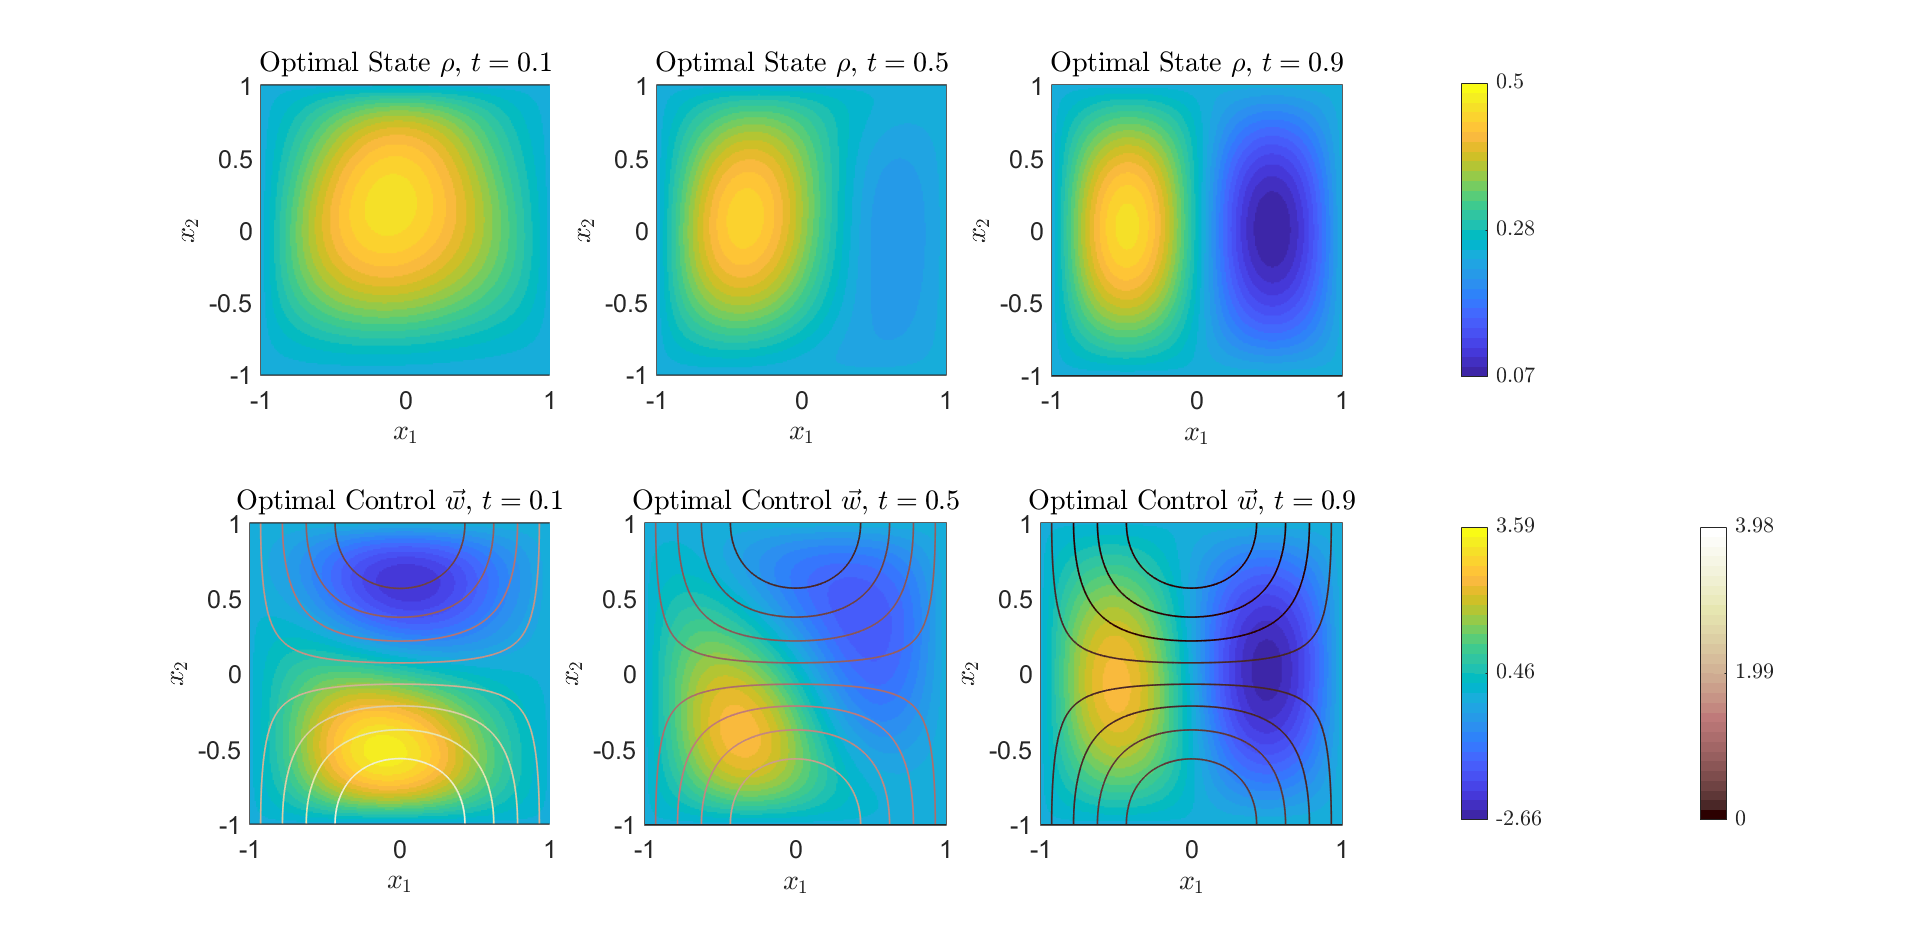
\includegraphics[scale=0.35]{SCDk0.png}
		\caption{Dirichlet Source Control: Optimal $\rho$ and optimal control for $\kappa = 0$ and $\beta = 10^{-3}$.} 
		\label{F2a}
	\end{figure}
	\begin{figure}[h]
		\centering
		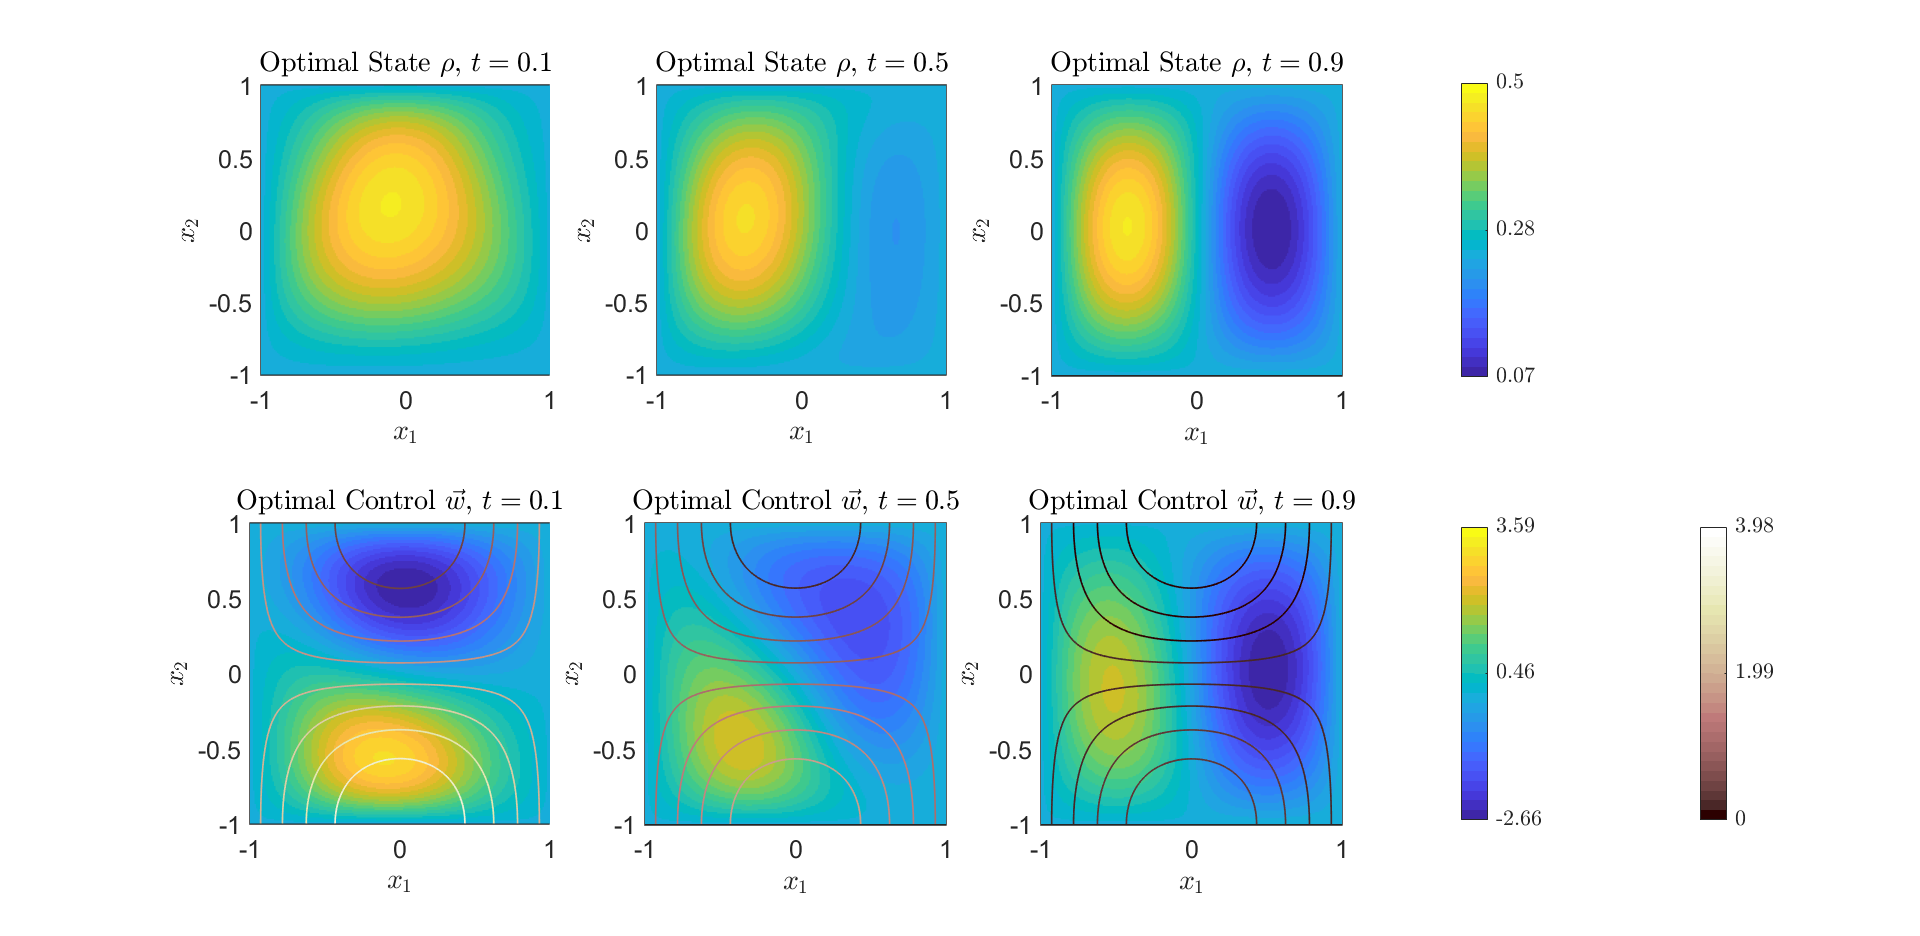
\includegraphics[scale=0.35]{SCDkn1.png}
		\caption{Dirichlet Source Control: Optimal $\rho$ and optimal control for $\kappa = -1$ and $\beta = 10^{-3}$.} 
		\label{F2b}
	\end{figure}
	\begin{figure}[h]
		\centering
		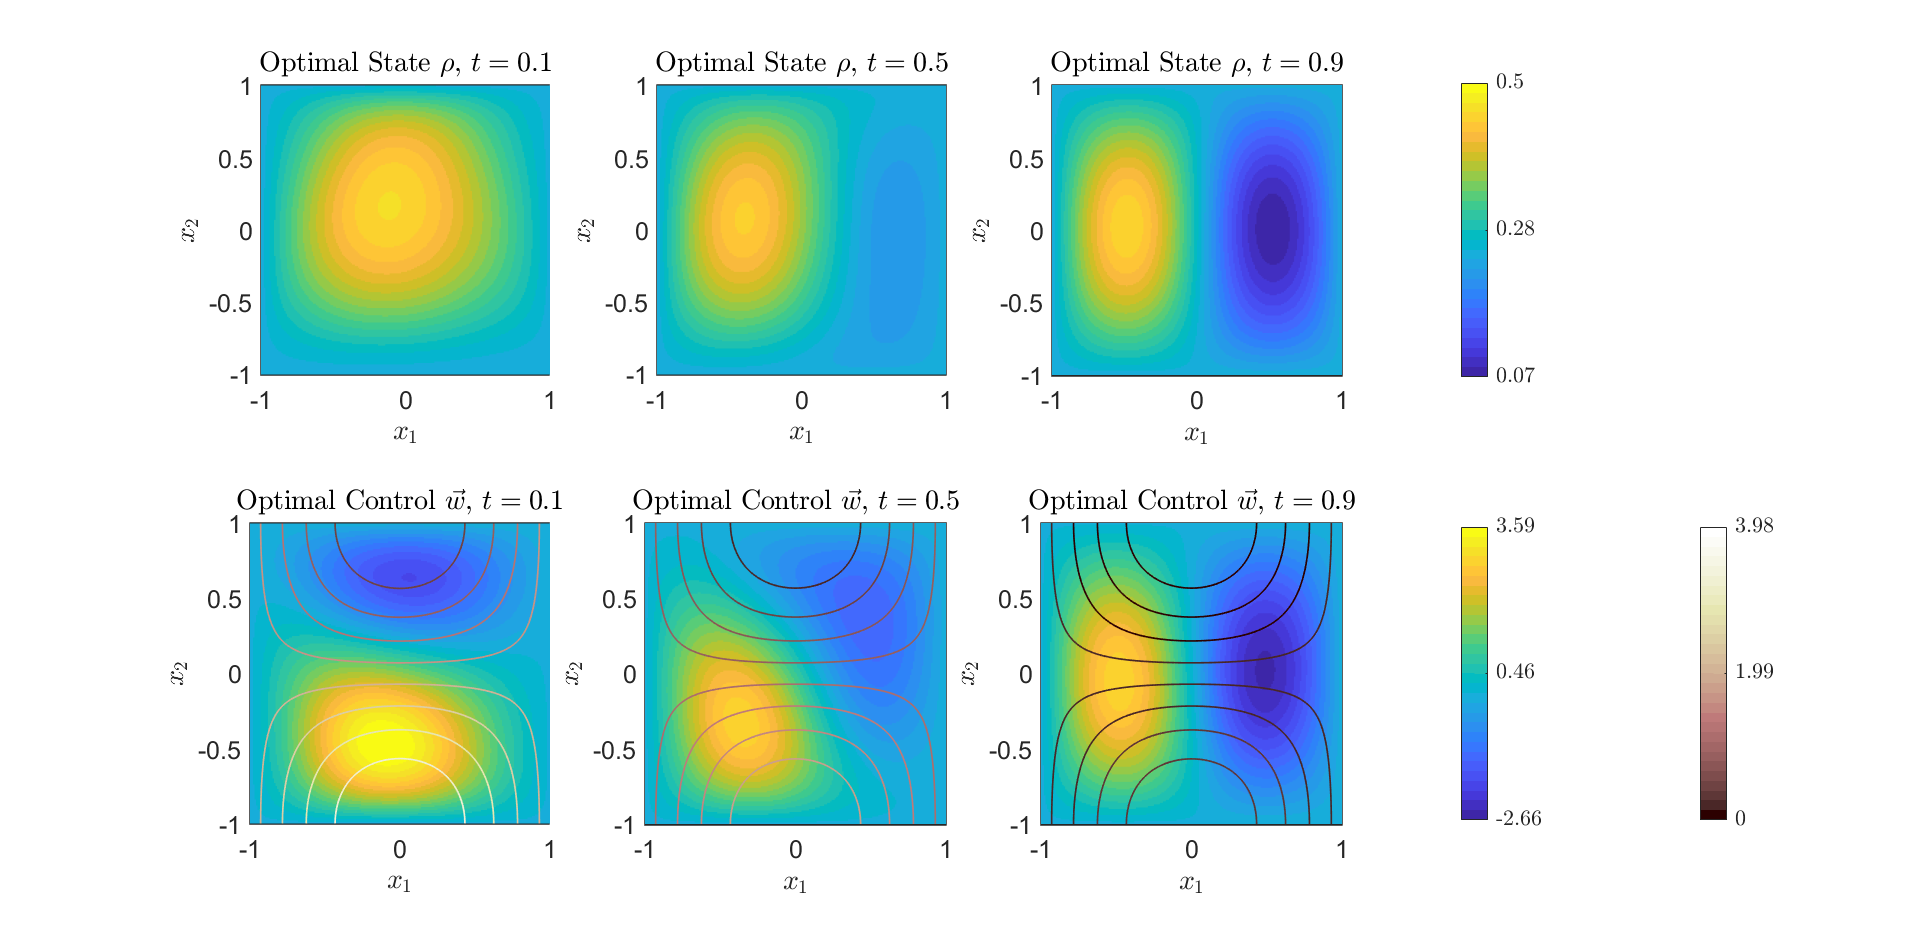
\includegraphics[scale=0.35]{SCDk1.png}
		\caption{Dirichlet Source Control: Optimal $\rho$ and optimal control for $\kappa = 1$ and $\beta = 10^{-3}$.} 
		\label{F2c}
	\end{figure}
	
	\section{Neumann Flow Control}
	We choose 
	\begin{align*}
		\rho_0 &= \frac{1}{4}\\
		V_{ext} &= \left(\left(x_1 + 0.3\right)^2 - 1\right)\left(\left(x_1-0.4\right)^2 - 0.5\right)
		\left(\left(x_2 + 0.3\right)^2 - 1\right)\left(\left(x_2-0.4\right)^2 - 0.5\right)\\
		\hr &= \frac{1}{4}(1-t) + t\frac{1}{1.3791}\exp{\left(-2\left(\left(x_1+0.2\right)^2 + \left(x_2+0.2\right)^2\right)\right)}
	\end{align*}
	We choose the domain $[-1,1]^2$ with a time horizon $(0,1)$. We have $N = 20$, $n = 11$. 
	For $\beta = 10^{-3}$, $\kappa = 1$ we get $\mathcal J_c = 0.0059$ (compare to $\beta = 10^3$ with $\mathcal J_{uc} = 0.0336$), for $\kappa = 0$, $\mathcal J_c = 0.0043$, and for $\kappa = - 1$ we get $\mathcal J_c = 0.0030$, (compare to $\beta = 10^3$ with $\mathcal J_{uc} = 0.0214$). Each of the problems takes around $180$ seconds to solve. The results can be seen in Figures \ref{F3a}, \ref{F3b} and \ref{F3c}. Note that mass is conserved.

	\begin{figure}[h]
		\centering
		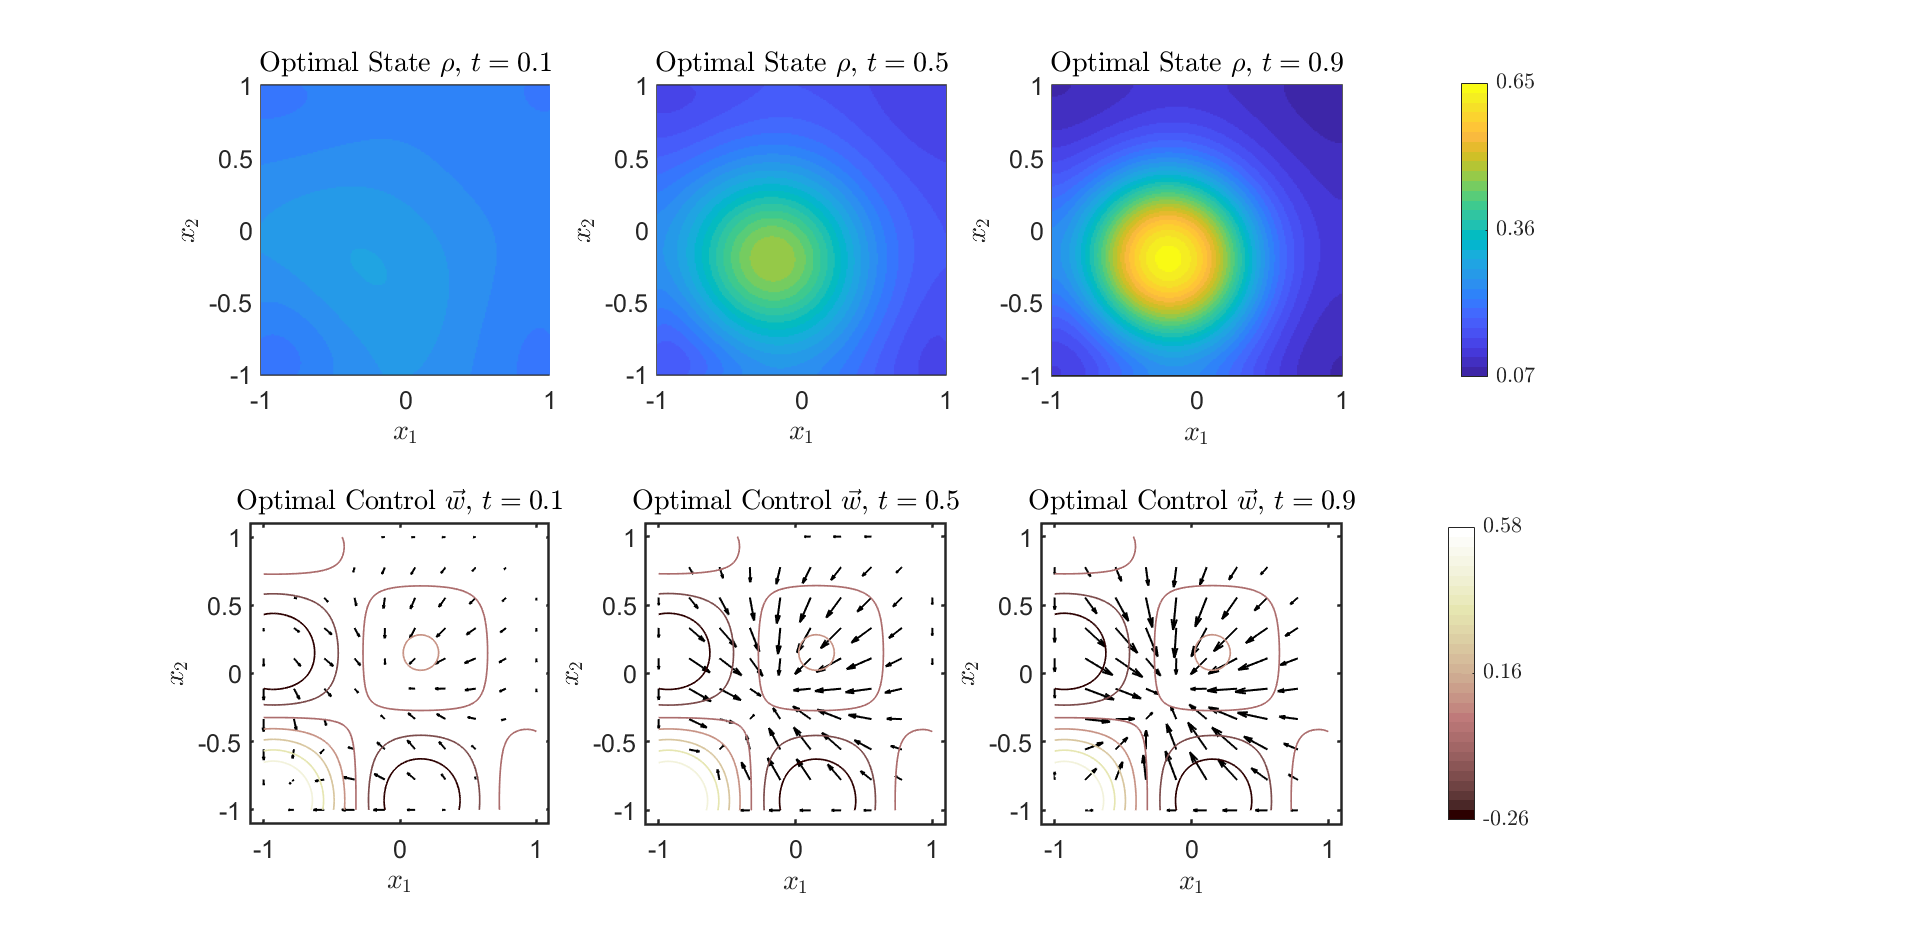
\includegraphics[scale=0.35]{FCNk0.png}
		\caption{Neumann Flow Control: Optimal $\rho$ and optimal control for $\kappa = 0$ and $\beta = 10^{-3}$.} 
		\label{F3a}
	\end{figure}
	\begin{figure}[h]
		\centering
		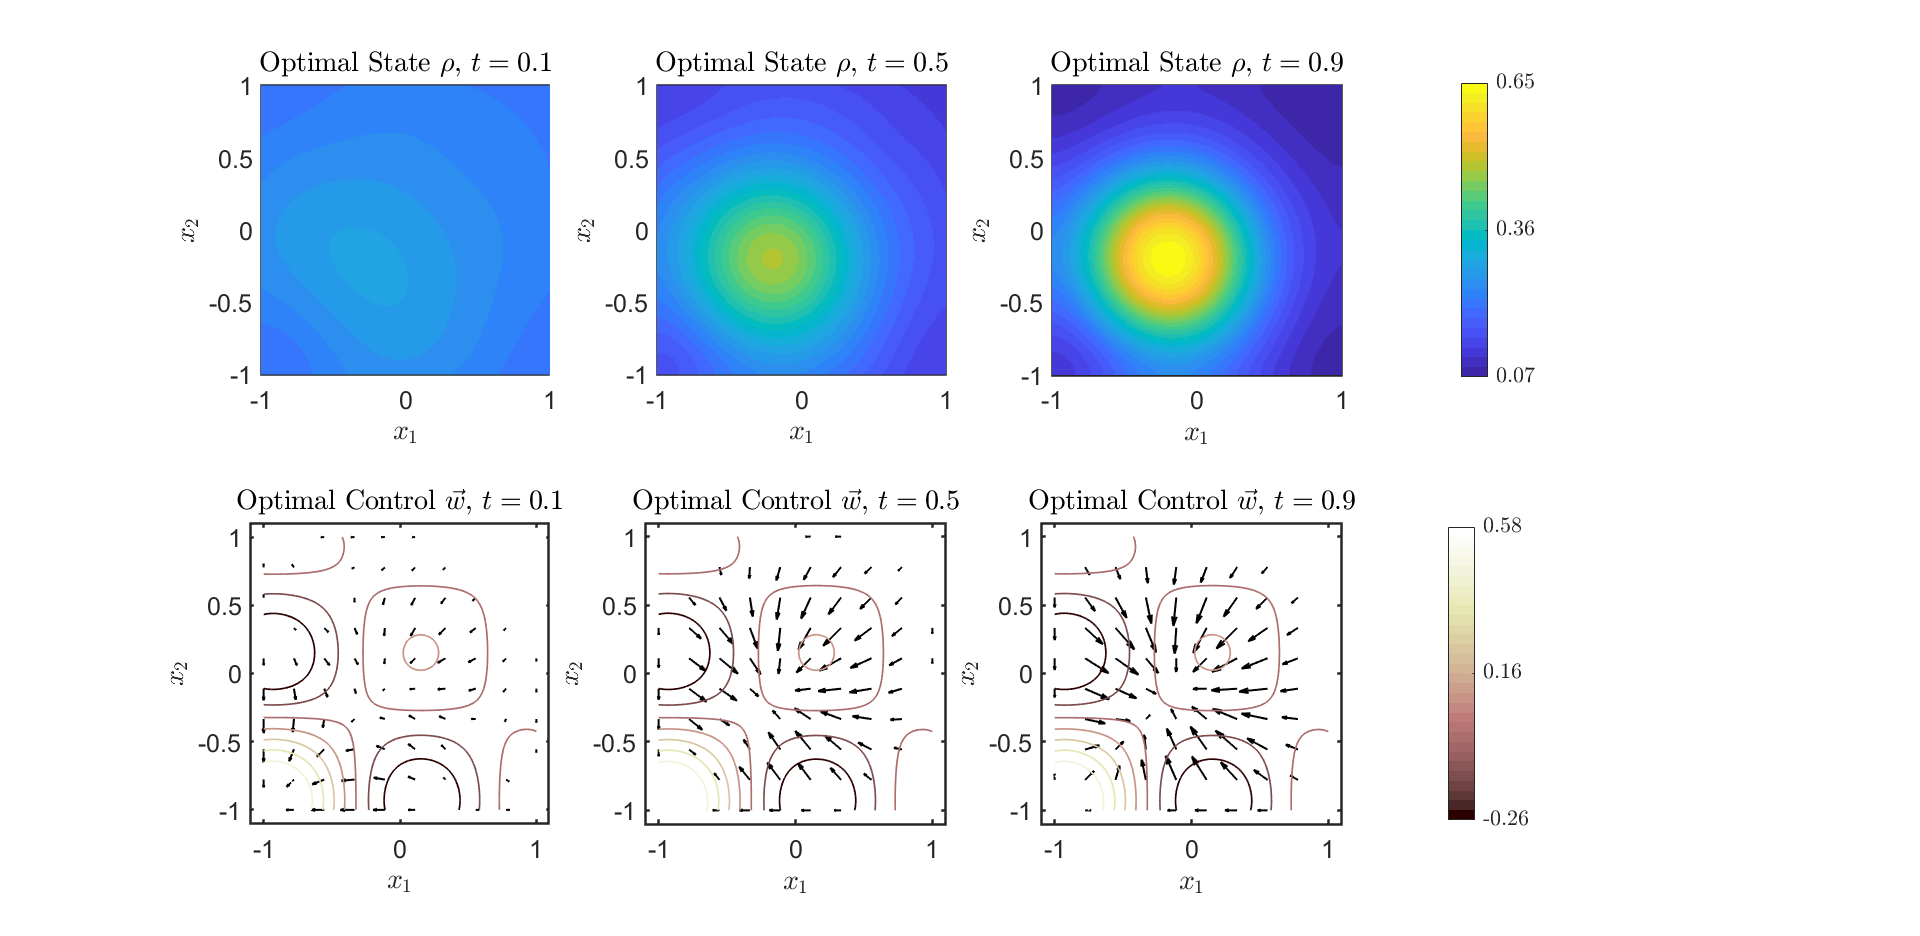
\includegraphics[scale=0.35]{FCNkn1.png}
		\caption{Neumann Flow Control: Optimal $\rho$ and optimal control for $\kappa = -1$ and $\beta = 10^{-3}$.} 
		\label{F3b}
	\end{figure}
	\begin{figure}[h]
		\centering
		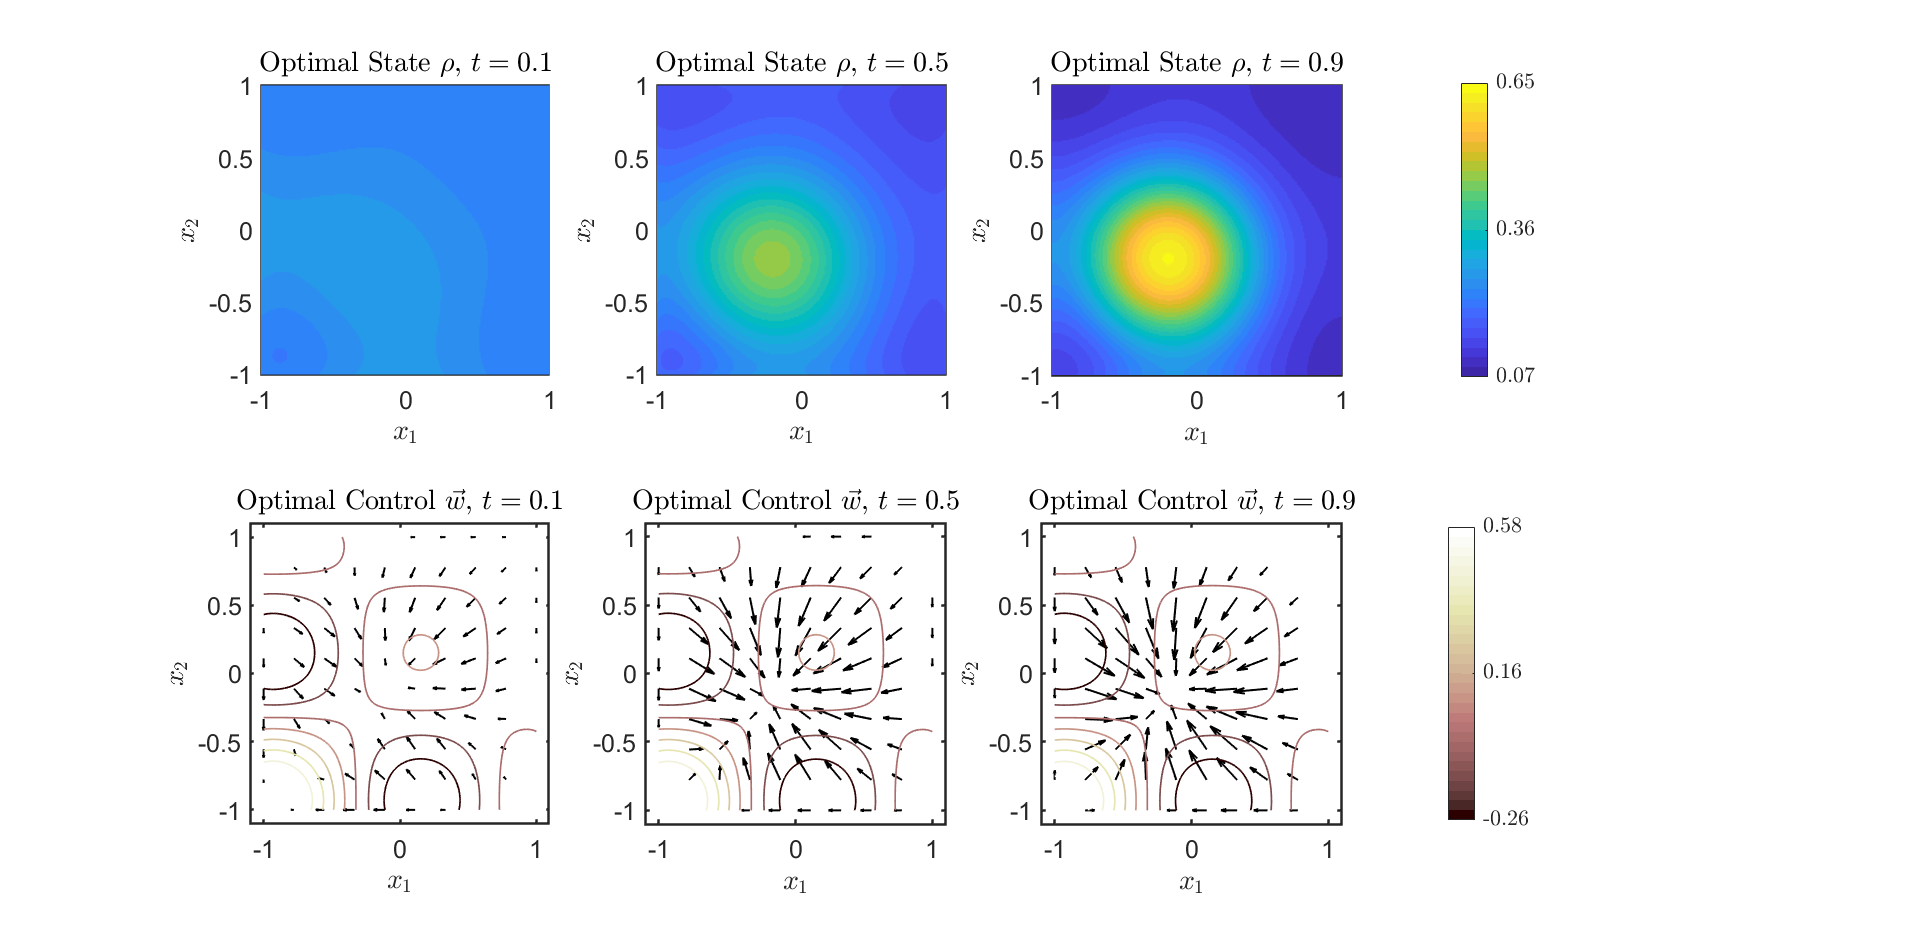
\includegraphics[scale=0.35]{FCNk1.png}
		\caption{Neumann Flow Control: Optimal $\rho$ and optimal control for $\kappa = 1$ and $\beta = 10^{-3}$.} 
		\label{F3c}
	\end{figure}
	
	\subsection{Dirichlet Flow Control}
	We add the following external potential to the above problem, see Figure \ref{F5V} 
	\begin{align*}
		V_{ext} = 10\sin\left(\frac{\pi x_1}{2}\right) \sin\left(\frac{\pi x_2}{3} - \frac{\pi}{2}\right)
	\end{align*}
	For $\beta = 10^{-3}$, $\kappa = 1$ we get $\mathcal J_c = 0.0130$, for $\kappa = 0$, $\mathcal J_c = 0.0106$, and for $\kappa = - 1$ we get $\mathcal J_c = 0.0113$. (Compare these to $\beta = 10^3$ with $\mathcal J_{uc} = 0.0898$) Each of the problems takes around $50$ seconds to solve. The results can be seen in Figures \ref{F5a}, \ref{F5b} and \ref{F5c}.
	
	
	\begin{figure}[h]
		\centering
		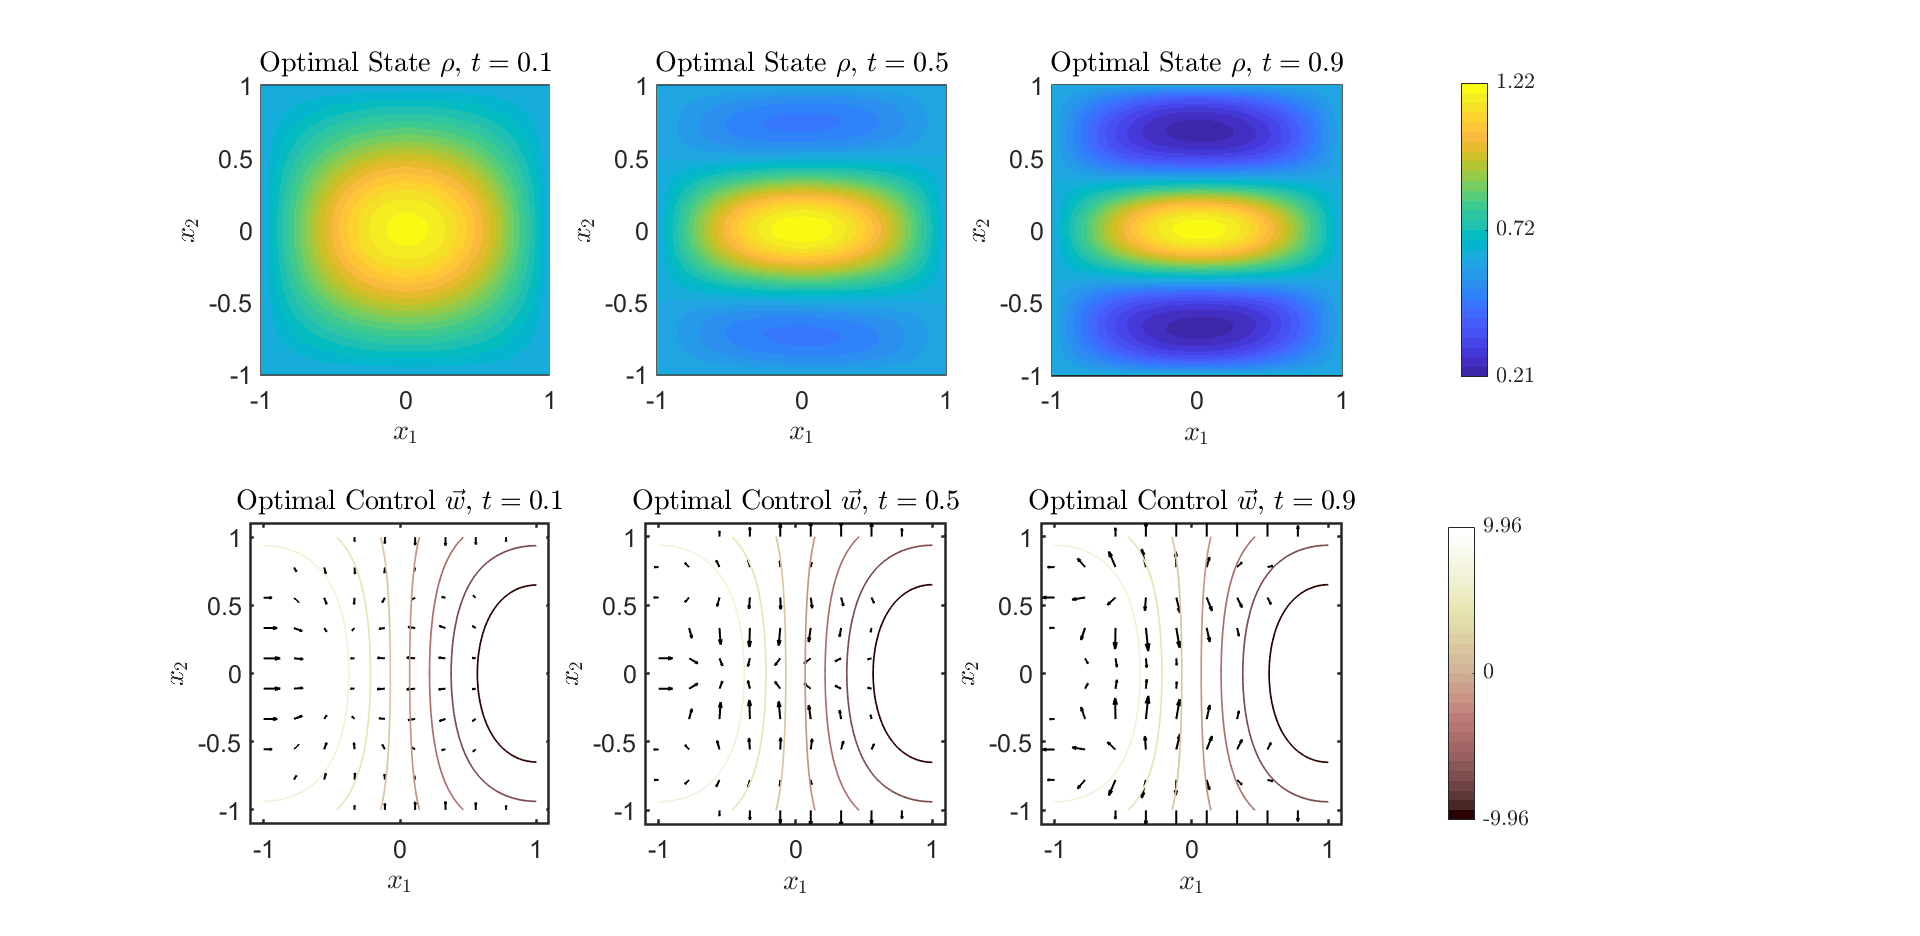
\includegraphics[scale=0.35]{FCDk0.png}
		\caption{Dirichlet Flow Control 2: Optimal $\rho$ and optimal control for $\kappa = 0$ and $\beta = 10^{-3}$.} 
		\label{F5a}
	\end{figure}
	\begin{figure}[h]
		\centering
		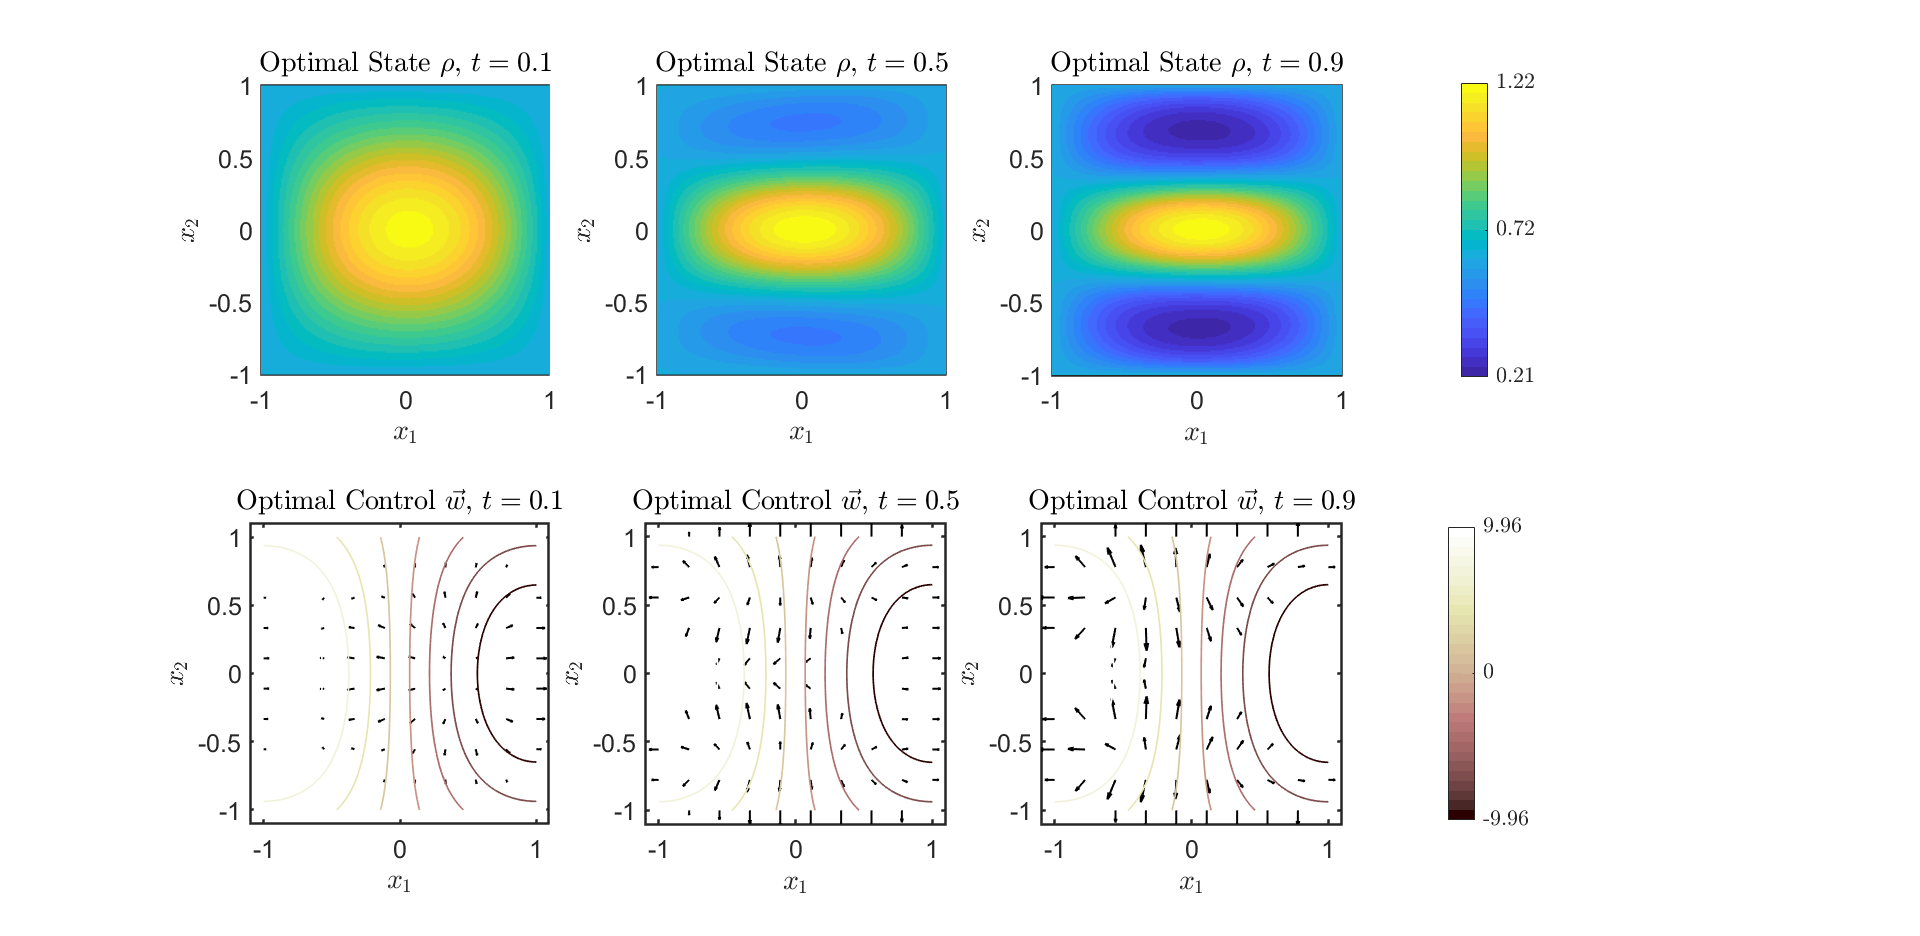
\includegraphics[scale=0.35]{FCDkn1.png}
		\caption{Dirichlet Flow Control 2: Optimal $\rho$ and optimal control for $\kappa = -1$ and $\beta = 10^{-3}$.} 
		\label{F5b}
	\end{figure}
	\begin{figure}[h]
		\centering
		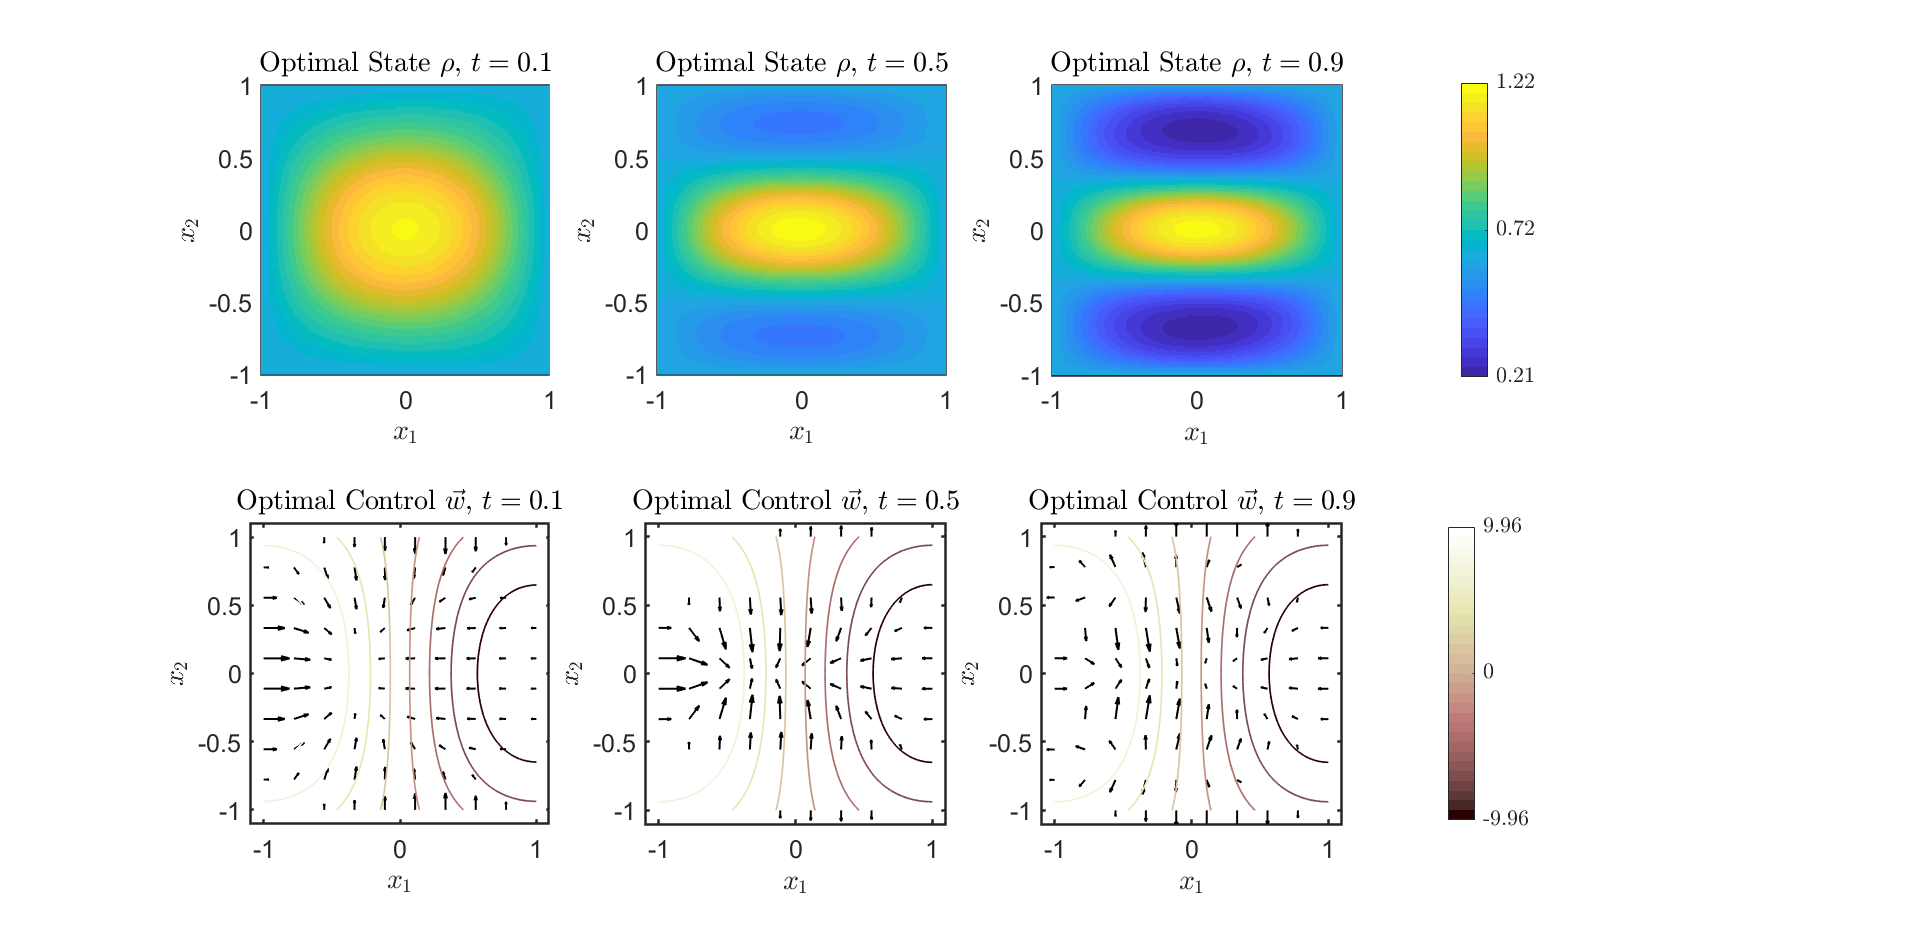
\includegraphics[scale=0.35]{FCDk1.png}
		\caption{Dirichlet Flow Control 2: Optimal $\rho$ and optimal control for $\kappa = 1$ and $\beta = 10^{-3}$.} 
		\label{F5c}
	\end{figure}







	\section*{Paper Example 3D}
	We choose 
	\begin{align*}
		\rho_0 &= 0.125\\
		V_{ext} &= ((x_1 + 0.3)^2 - 1)((x_1 - 0.4)^2 - 0.5)\\
		&\quad ((x_2 + 0.3)^2 - 1)((x_2 - 0.4)^2 - 0.5)((x_3 + 0.3)^2 - 1)((x_3 - 0.4)^2 - 0.5)\\
		\hr &= 0.125(1-t) + t\left(\frac{\pi}{4}\right)^3\cos\left(\frac{\pi x_1}{2}\right)\cos\left(\frac{\pi x_2}{2}\right)\cos\left(\frac{\pi x_3}{2}\right)
	\end{align*}
	The external potential is shown in Figure \ref{F1}.
%	\begin{figure}[h]
%		\centering
%		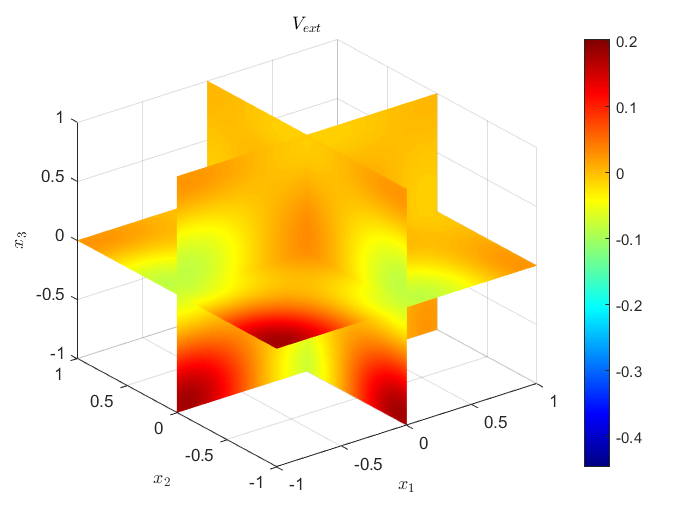
\includegraphics[scale=0.7]{Vext3D.png}
%		\caption{External Potential $V_{ext}$} 
%		\label{F1}
%	\end{figure}
	
	For $N = 20$ and $n = 11$, with $\beta = 10^{-3}$ we get for $\kappa = 0$, $\mathcal J_c = 0.0078$, with $\mathcal J_1 = 0.0071$ and $\mathcal J_2 = 8.5034$.
	This can be compared to $\mathcal J_{uc} = 0.0195$ from the computed forward problem with $\w = \vec 0$.\\
	For $\kappa = 1$, we get that $\mathcal J_c = 0.0102$, with $\mathcal J_1 = 0.0097$, $\mathcal J_2 = 10.7306$. Compare to $\mathcal J_{uc} = 0.0232$. \\
	For $\kappa = -1$ we have $\mathcal J_c = 0.0059$, $\mathcal J_1 = 0.0054$, $\mathcal J_2 = 6.4039$. Compare to $\mathcal J_{uc} = 0.0477$.
	While the forward problem takes around $12$ minutes to solve, the optimal control problem with Newton-Krylov takes about 35 hours for 10 outer iterations, which is enough for convergence. Mass is conserved to $10^{-4}$. The results can be seen in Figures \ref{F2}, \ref{F3} and \ref{F4}. 
	\\
	\\
	The controls are plotted in Figures \ref{F5}, \ref{F6} and \ref{F7}. They are all normalized to the maximum over all three controls and scaled by a factor of $2$ for visibility. The figures are still not good though. I am not sure how the scaling works -- $\kappa = 0$ should have way smaller arrows by that logic.

	

	\begin{figure}[h]
		\centering
		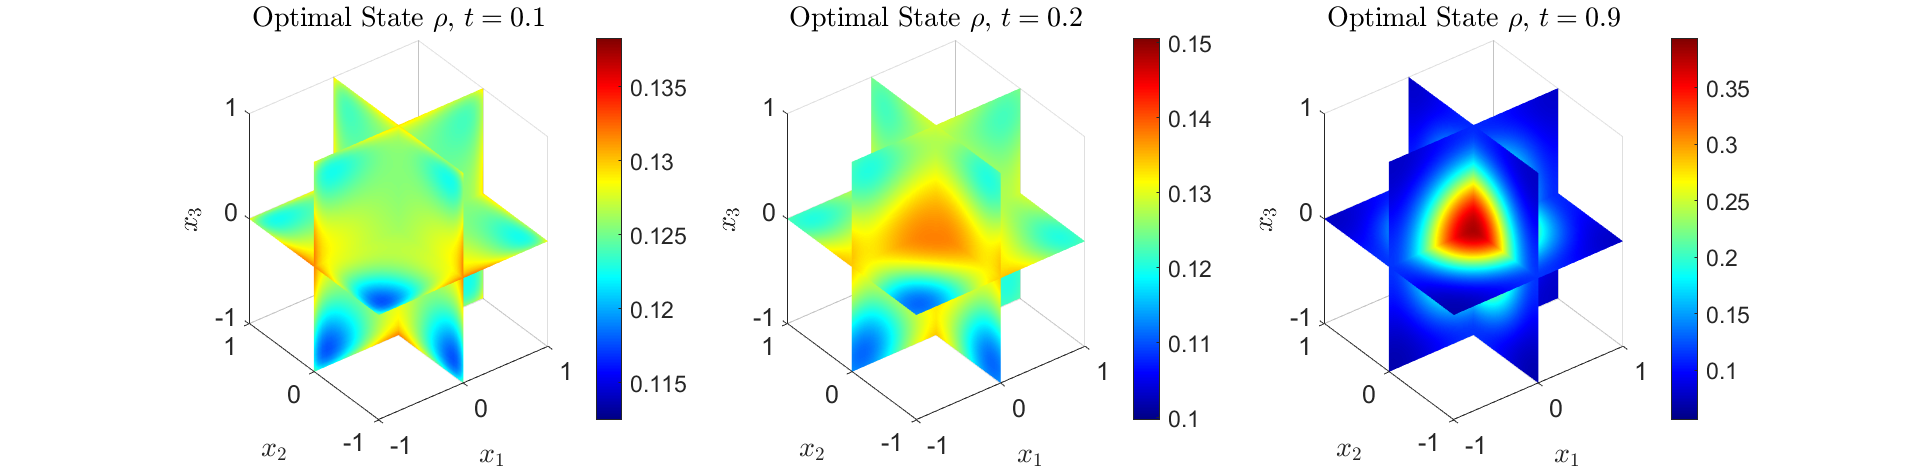
\includegraphics[scale=0.35]{rhok1.png}
		\caption{Optimal state $\rho$ for $\kappa = 1$.} 
		\label{F2}
	\end{figure}
	\begin{figure}[h]
		\centering
		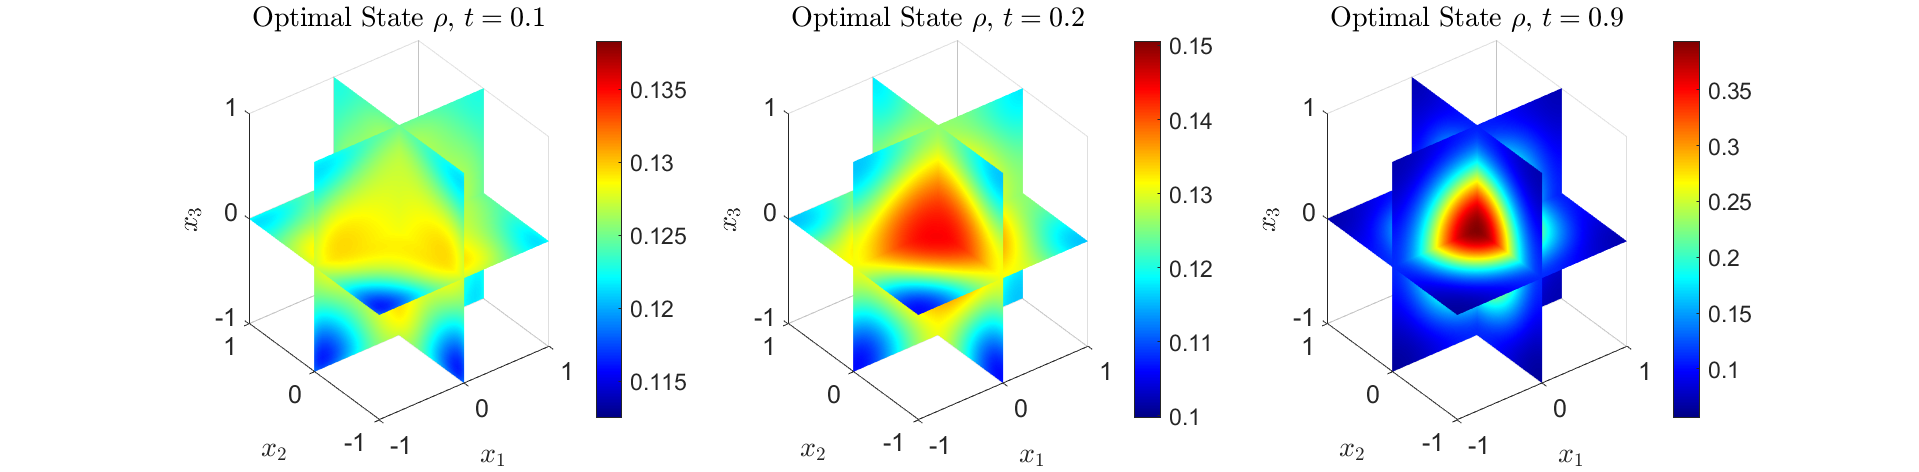
\includegraphics[scale=0.35]{rhok0.png}
		\caption{Optimal state $\rho$ for $\kappa = 0$.} 
		\label{F3}
	\end{figure}
	\begin{figure}[h]
		\centering
		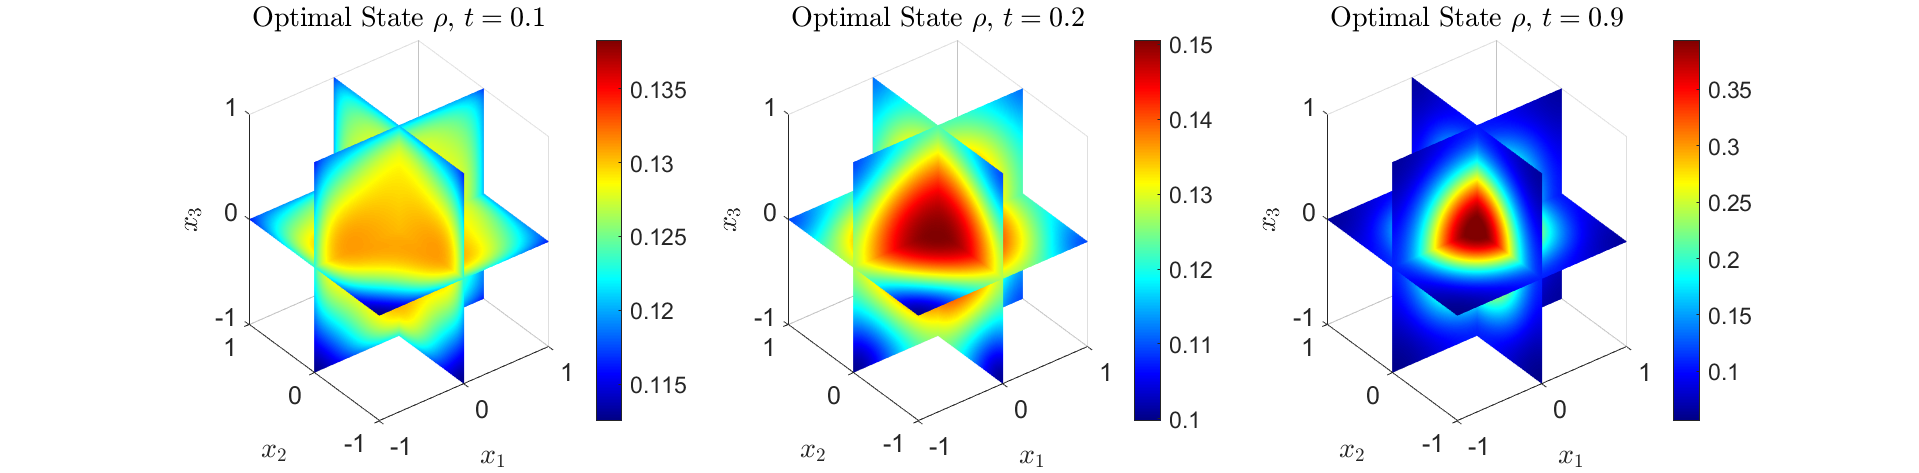
\includegraphics[scale=0.35]{rhokn1.png}
		\caption{Optimal state $\rho$ for $\kappa = -1$.} 
		\label{F4}
	\end{figure}
%	
	\begin{figure}[h]
		\centering
		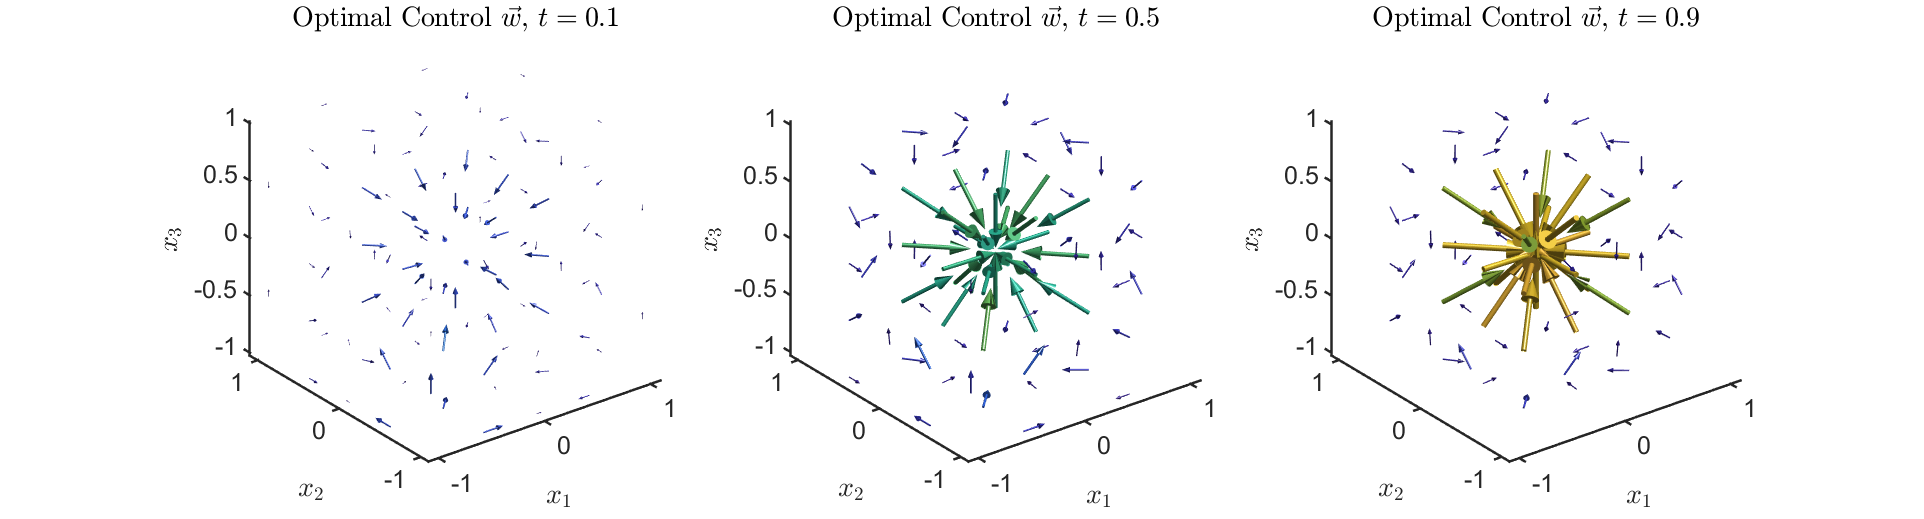
\includegraphics[scale=0.35]{Controlk1.png}
		\caption{Optimal control $\w$ for $\kappa = 1$.} 
		\label{F5}
	\end{figure}
	\begin{figure}[h]
		\centering
		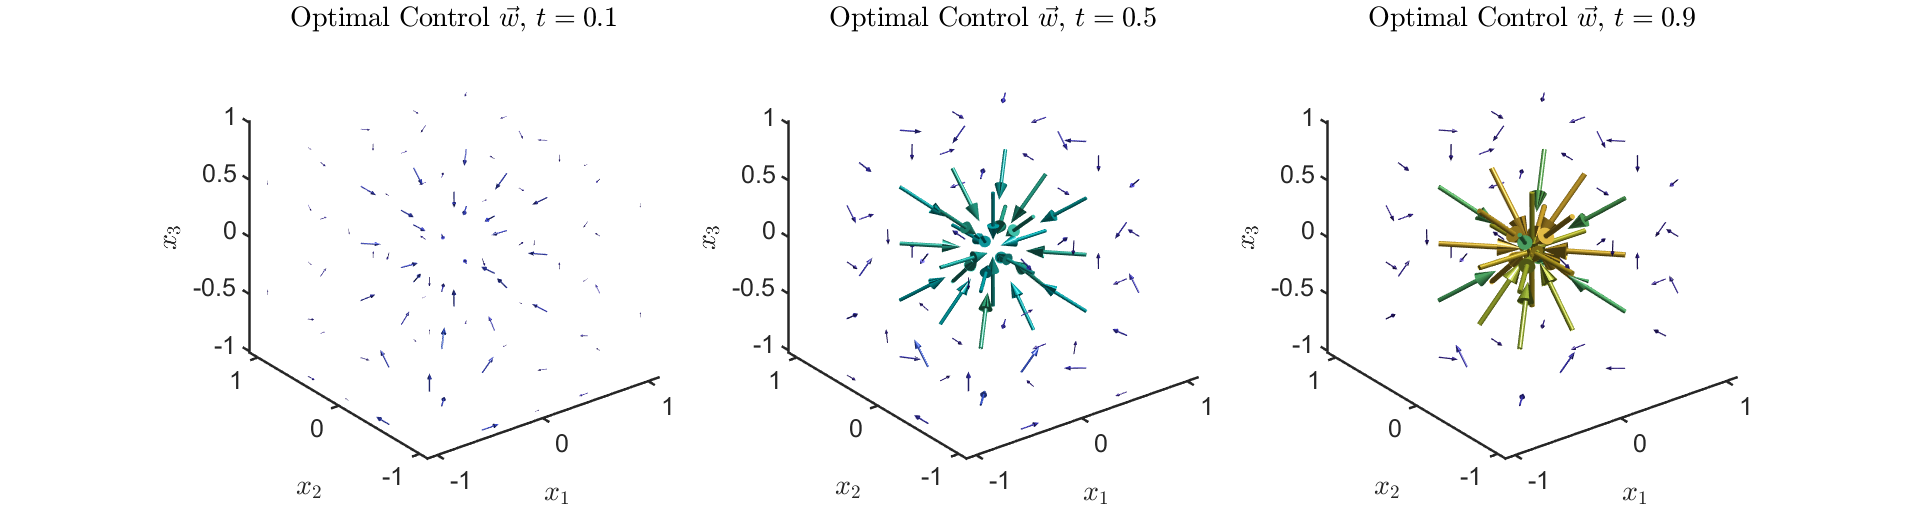
\includegraphics[scale=0.35]{Controlk0.png}
		\caption{Optimal control $\w$ for $\kappa = 0$.} 
		\label{F6}
	\end{figure}
	\begin{figure}[h]
		\centering
		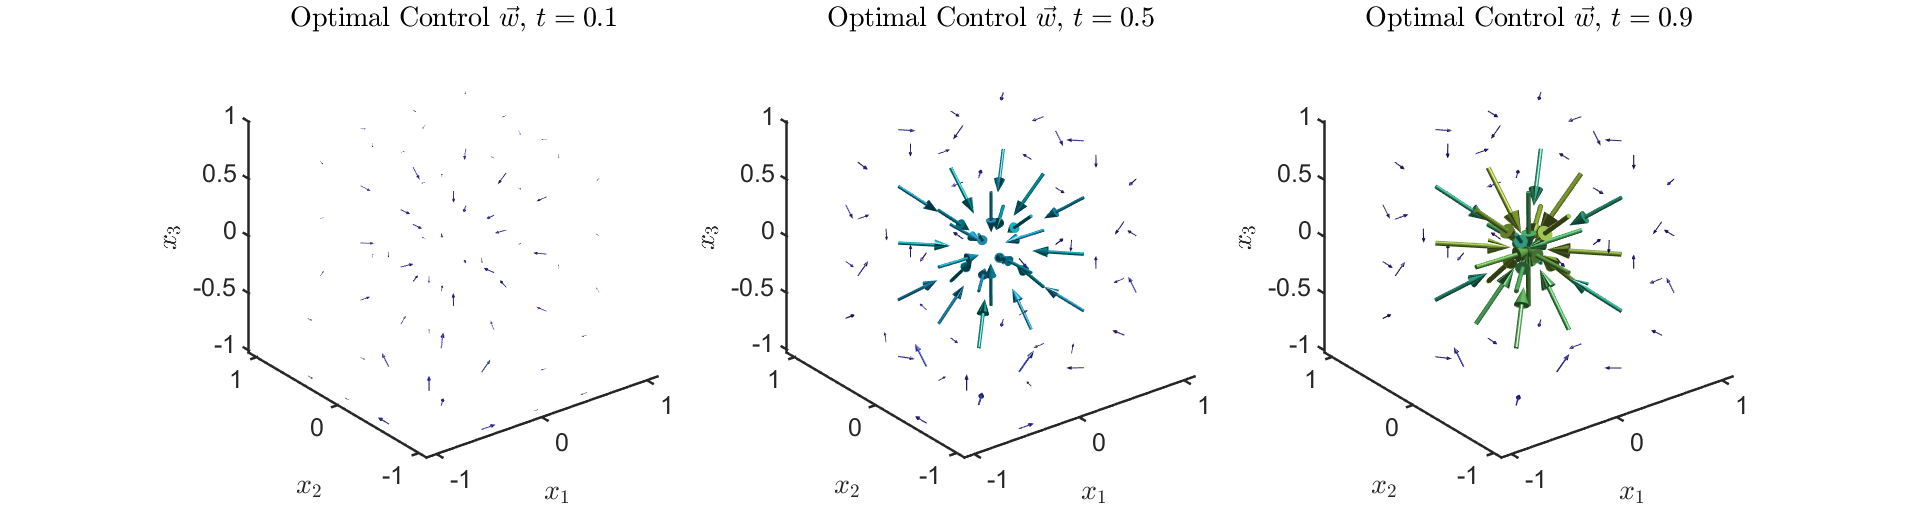
\includegraphics[scale=0.35]{Controlkn1.png}
		\caption{Optimal control $\w$ for $\kappa = -1$.} 
		\label{F7}
	\end{figure}
%	
%	\begin{figure}[h]
%		\centering
%		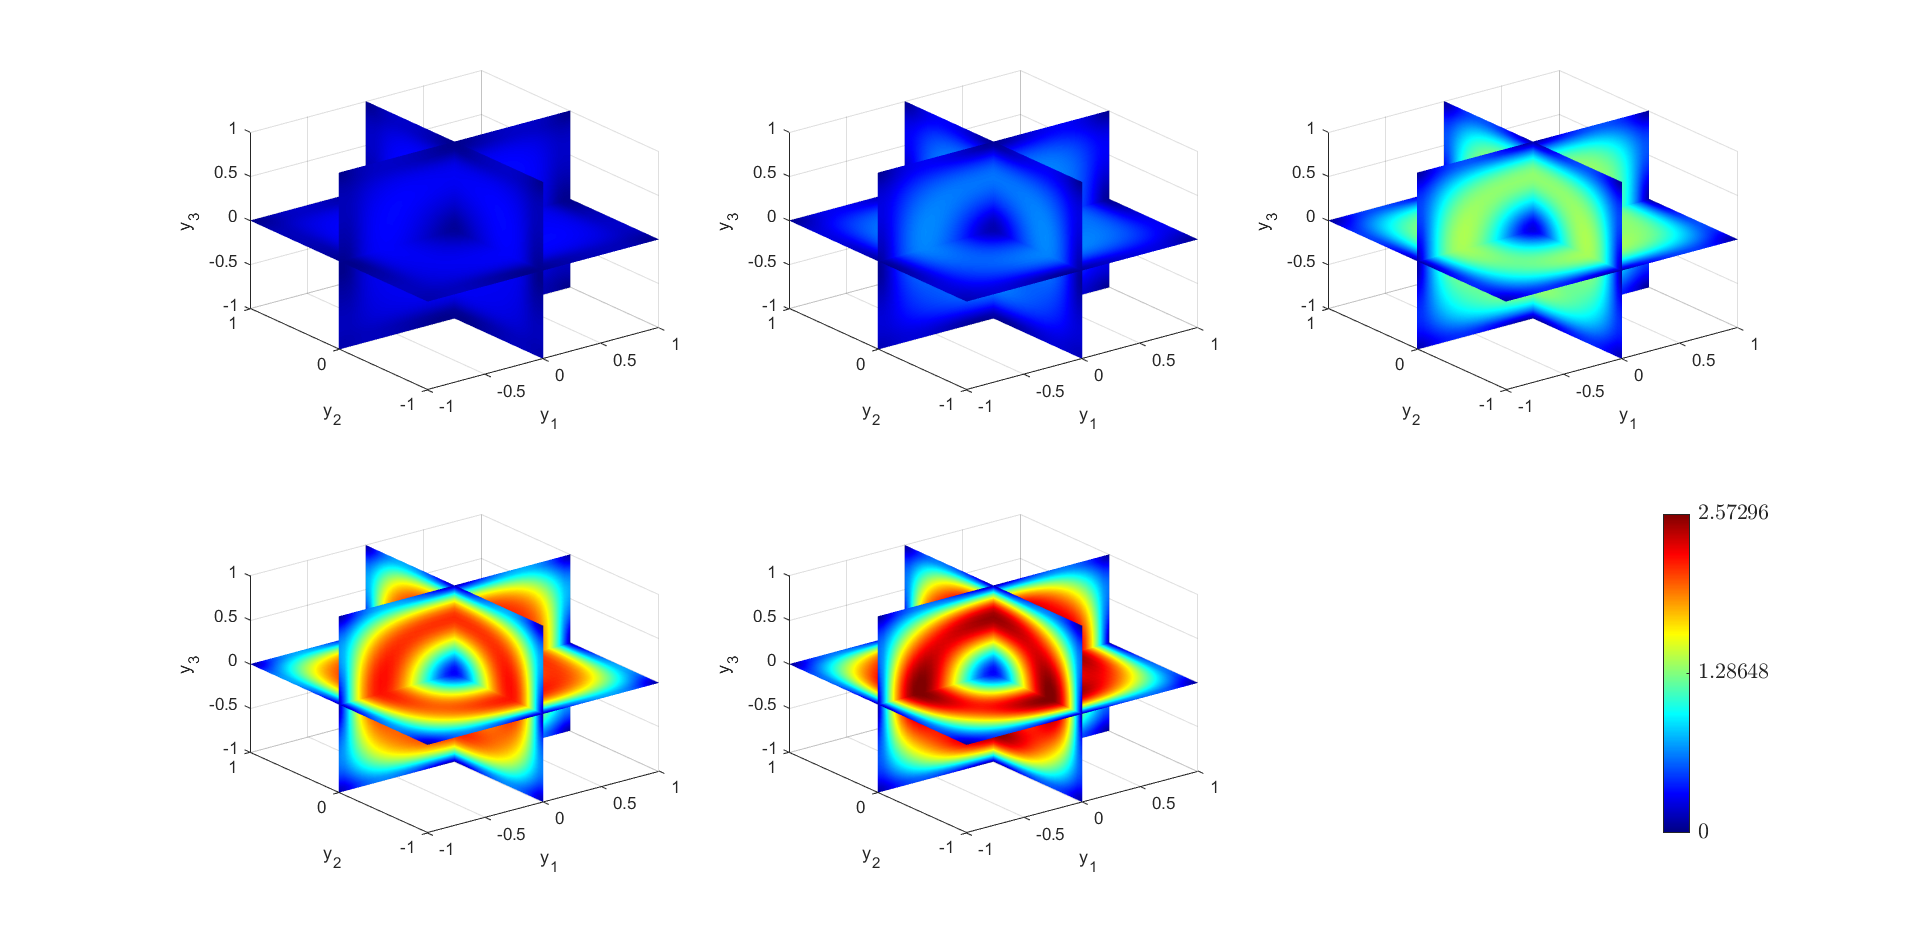
\includegraphics[scale=0.35]{wNormk1.png}
%		\caption{Norm of the optimal control $\w$, at times 1, 3, 5, 7 and 9 for $\kappa = 1$.} 
%		\label{F4a}
%	\end{figure}
%	
%	\begin{figure}[h]
%		\centering
%		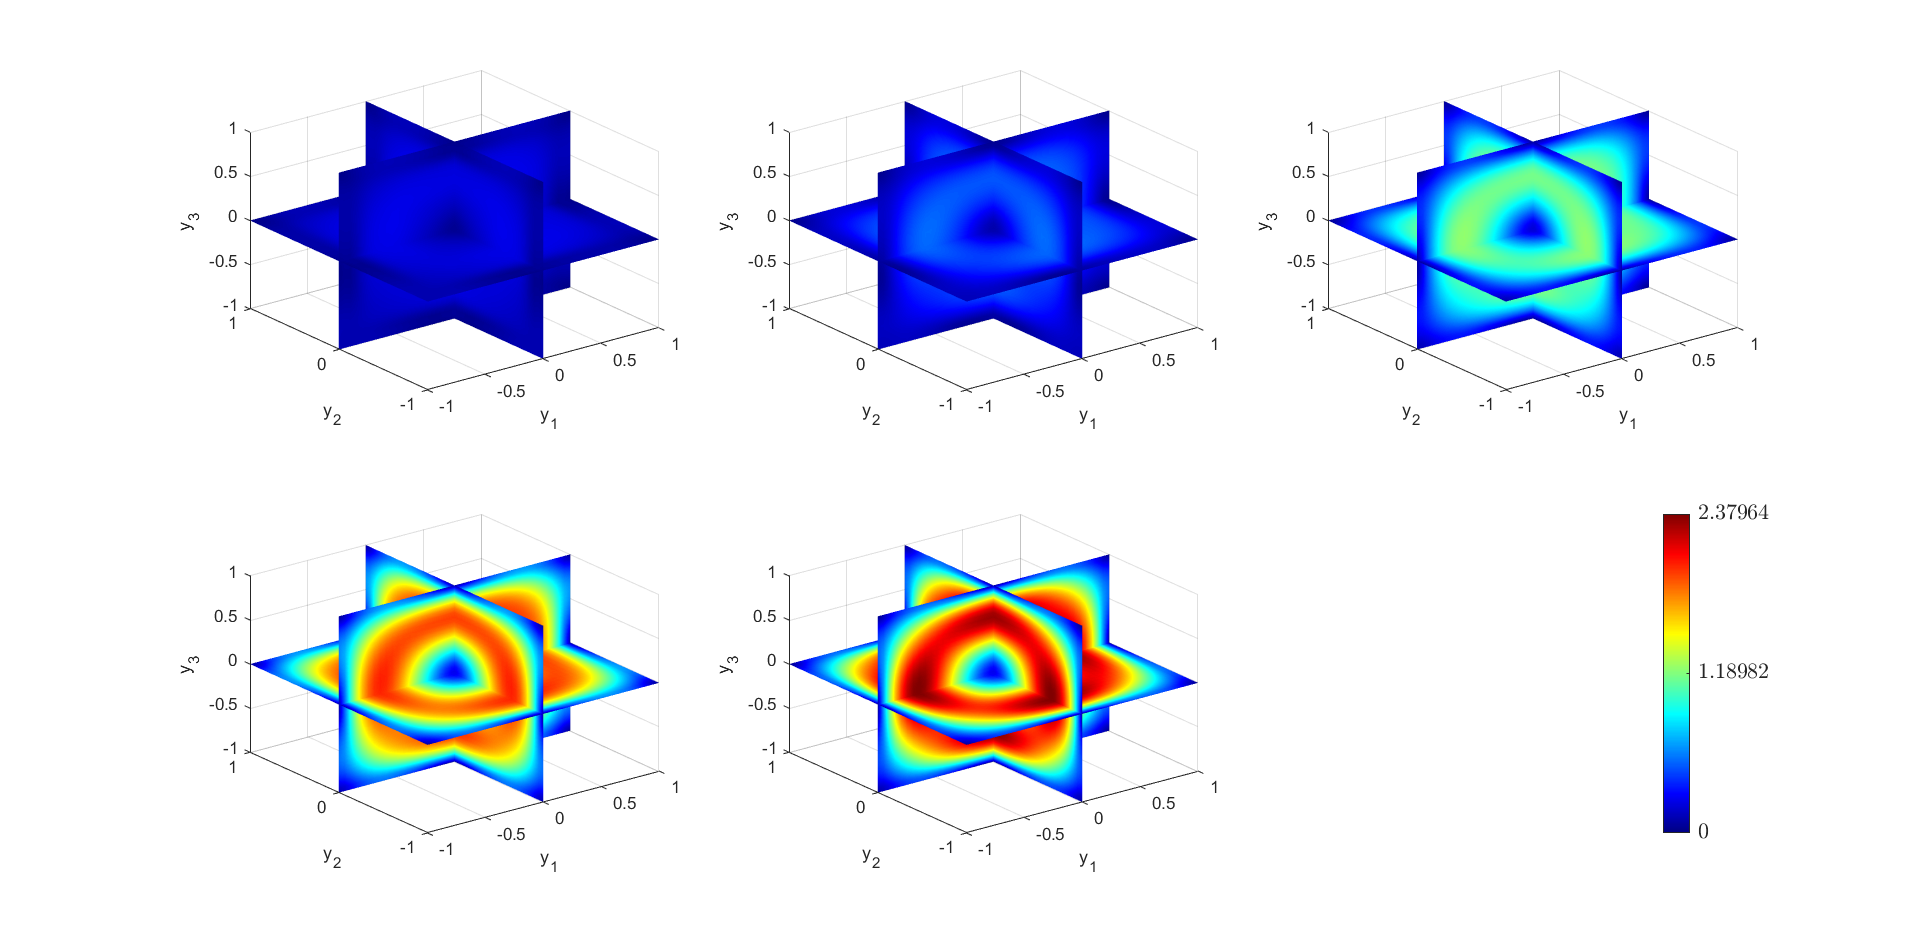
\includegraphics[scale=0.35]{wNormk0.png}
%		\caption{Norm of the optimal control $\w$, at times 1, 3, 5, 7 and 9 for $\kappa = 0$.} 
%		\label{F4b}
%	\end{figure}
%	\begin{figure}[h]
%		\centering
%		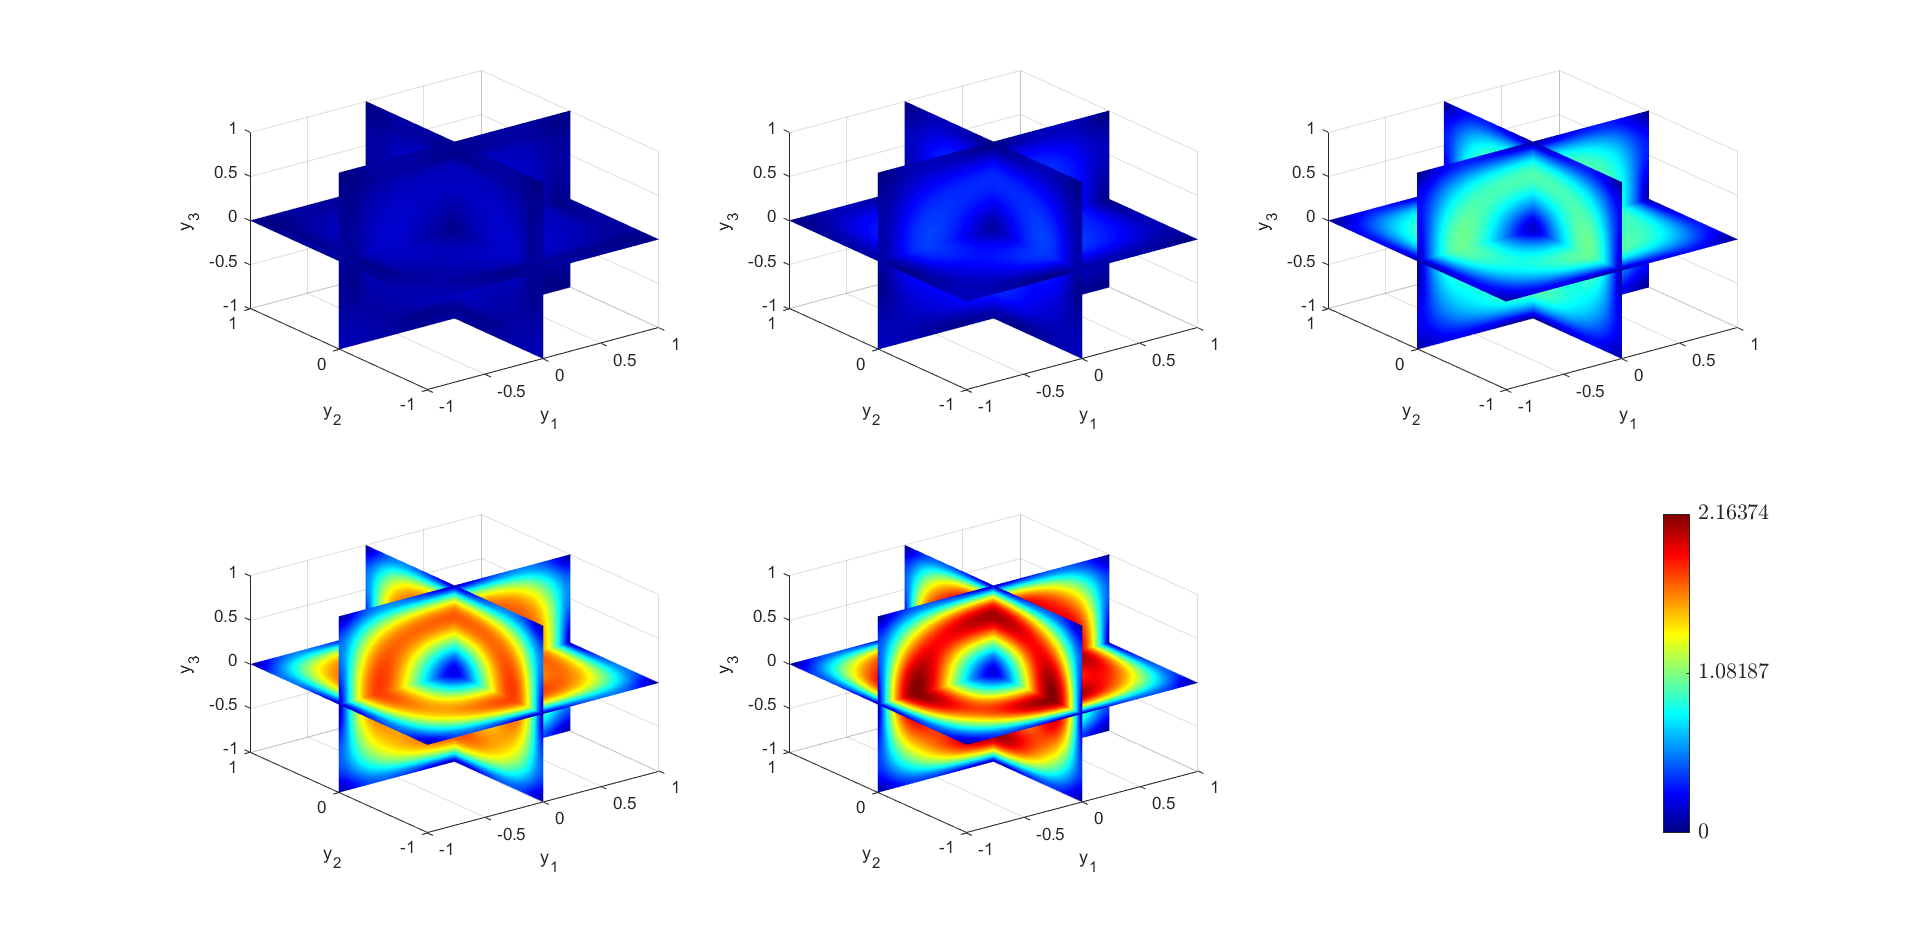
\includegraphics[scale=0.35]{wNormkn1.png}
%		\caption{Norm of the optimal control $\w$, at times 1, 3, 5, 7 and 9 for $\kappa = -1$.} 
%		\label{F4c}
%	\end{figure}
%	
	
\end{document}